\documentclass[11pt]{article}
\usepackage[utf8]{inputenc}
\usepackage{amsmath, amsthm, amssymb}
% add "showframe" param to geometry package below to see margin lines
\usepackage[letterpaper, margin=1in]{geometry}
\usepackage{microtype}
\usepackage[shortlabels]{enumitem}
\usepackage{biblatex}
\usepackage{mathtools}
\usepackage{amssymb}
\usepackage{float}
\usepackage{commath}
\usepackage{color, soul}
\usepackage{wrapfig}
\usepackage{xfrac}
\usepackage{xcolor}
\usepackage{hyperref}
\hypersetup{
    colorlinks,
    linkcolor={blue},
    citecolor={blue},
    urlcolor={blue}
}
\usepackage[colorinlistoftodos,textsize=tiny]{todonotes}
\usepackage{comment}
\usepackage{setspace}
\usepackage{titling}


\let\comment\todo
\newcommand{\frank}[1]{\comment[nolist,color=blue!40]{@frank\\ #1}}
\newcommand{\david}[1]{\comment[nolist,color=orange!40]{@david\\ #1}}
\newcommand{\katie}[1]{\comment[nolist,color=green!40]{@katie\\ #1}}
\newcommand{\question}[1]{\comment[nolist,color=red!40]{#1}}

\addbibresource{main.bib}

\newtheorem{theorem}{Theorem}[section]
\newtheorem{corollary}{Corollary}[theorem]
\newtheorem{lemma}[theorem]{Lemma}
\newtheorem{alg}[theorem]{Algorithm}
\newtheorem{claim}[theorem]{Claim}

\theoremstyle{definition}
\newtheorem{definition}{Definition}[section]

\theoremstyle{definition}
\newtheorem{subroutine}{Subroutine}

\theoremstyle{definition}
\newtheorem{example}{Example}[section]

% Commonly used symbols
\newcommand{\R}{\mathbb{R}}
\newcommand{\fu}{f^{\mu}}
\newcommand{\nfi}{\nabla f_i}
\newcommand{\nfiu}{\nabla \fu_i}
\newcommand{\biu}{b_{i}^{\mu}}
\newcommand{\gij}{\gamma_{ij}}
\newcommand{\geu}{\gamma_e^{\mu}}
\newcommand{\giij}{\gamma_{ij}^{\mu}}
\newcommand{\vnott}{V \setminus t}
\newcommand{\din}{\delta^{\text{in}}}
\newcommand{\dout}{\delta^{\text{out}}}
\newcommand{\vsrc}{V^{s}}
\newcommand{\vsink}{V^{t}}
\newcommand{\vz}{V^{0}}
\newcommand{\fp}{(f,\mu)}
\newcommand{\fiju}{f_{ij}^{\mu}}

\newcommand{\tf}{\textsc{Tight-Flow}}
\newcommand{\ppn}{\textsc{Produce-Plentiful-Node}}
\newcommand{\filtration}{\textsc{De-Isolation}}
\newcommand{\es}{\textsc{Elementary-Step}}

\newcommand{\xands}{X \cap S}
\newcommand{\xnots}{X \setminus S}
\DeclareMathOperator{\Ex}{Ex}
\DeclareMathOperator{\Def}{Def}

\newcommand{\rewrite}[1]{\textcolor{red}{#1}}
\newcommand{\cbb}[1]{\textcolor{orange}{#1}}
\renewcommand{\todo}[1]{\hl{TODO: #1}}

\newcommand{\lpeq}[1] {
\begin{equation*}
\begin{aligned}
#1
\end{aligned}
\end{equation*}
}
\newcommand{\lpone}[3] {
& \underset{}{\text{#1}}
&& #2 \\
& \text{s.t.}
&& #3 
}
\newcommand{\lptwo}[4] {
\lpone{#1}{#2}{#3}\\
&&& #4
}
\newcommand{\lpthree}[5] {
\lptwo{#1}{#2}{#3}{#4}\\
&&& #5
}

\newif\ifLAYOUTA
\newif\ifLAYOUTB
\LAYOUTAtrue
\LAYOUTBfalse

\ifLAYOUTA
\setlength{\droptitle}{-4em}   % This is your set screw
\fi


\title{Strongly Polynomial Algorithms for Generalized Flow Maximization}
\author{Francis Cangialosi \\ \texttt{frankc@mit.edu} \and Katie Lewis \\ \texttt{kmlewis@mit.edu} \and David Palmer \\ \texttt{drp@mit.edu}}
\date{}

\begin{document}
\maketitle
\vspace{-0.3cm}

\section{Introduction}\label{sec:intro}
	\subsection{Problem Definition}\label{sec:problem}
	Let $G = (V,E)$ be a graph. As in the ordinary maximum flow problem,
    the generalized maximum flow problem aims to maximize the
	total flow delivered to the sink node $t \in V$. Each edge $e$
    is endowed with a gain factor $\gamma_e > 0$, which scales
	the flow passing through that edge. Gains might represent exchange rates between currencies
	or dissipation of a physical quantity. Setting $\gamma_e \equiv 1$
    recovers the ordinary maximum flow problem.
    
    The generalized maximum
	flow problem lacks several nice properties of the ordinary
	maximum flow problem, which makes it more challenging to solve. For example,
	the generalized problem is usually thought to be non-integral and,
	due to the gain factors, the total supply is not necessarily equal to the total
	demand. Additionally, the maximum flow--minimum cut theorem no longer applies
	since the flow along a path is not equal at every edge along that path.
    
	Until recently, the best known algorithms were all weakly polynomial. In
	2013, Végh developed the first strongly polynomial algorithm~\cite{Vegh2013}
% 	(i.e. one that depends only on the number of nodes and edges in the graph,
% 	and is independent of the size of their values).
    In 2017, Olver and Végh
	built on this work and developed an algorithm~\cite{Olver2017}
	that is faster than Végh's original algorithm by a factor of
	almost $O(n^2)$, resulting in a running time that is as fast as the best
	weakly polynomial algorithms even for small parameter values. 
	\ifLAYOUTA
	\else
	\rewrite{These
	algorithms take advantage of the structural similarities between the
	generalized maximum flow problem and the minimum cost flow problem by
	adapting techniques from well-known combinatorial min cost flow algorithms,
namely~\cite{Orlin1988}.}
	\fi
    
	\subsection{Structure and Contributions of the Paper}\label{sec:structure}
	In this paper, we aim to
	familiarize the reader with the recent algorithmic developments for the
	generalized flow maximization problem and provide intuition for the techniques
	used to achieve a strongly polynomial result. In Section~\ref{sec:prelim}, we formalize
    the problem as a linear program and give an overview of the notation
	used in the rest of the paper. In Section~\ref{sec:motivate}, we develop the key techniques
	both algorithms use to achieve a strongly polynomial bound for this
	problem. In Section~\ref{sec:2013}, we describe Végh's original $O(n^3m^2 \log n)$ strongly
	polynomial algorithm developed in 2013 and provide intuition for the running
	time analysis. 
	In Section~\ref{sec:2017}, we describe Olver and
	Végh's faster $O((m + n\log n)mn\log(n^2 / m))$ algorithm and highlight key
	aspects of the analysis that led way to the improved running time efficiency.
	Finally, in Section~\ref{sec:discussion}, \rewrite{we conclude}.
	\question{A little abrupt. Is there a better way to say this?}
    
\section{Preliminaries}\label{sec:prelim}

	\subsection{Network Notation}\label{sec:notation}
	%An instance of the generalized flow problem is specified as	
	Let $G=(V,E)$ be a directed graph with $n=\abs{V}$ and $m=\abs{E}$ (assume
	$m \geq n$), $t \in V$ be a sink node and $\gamma \in \R_{>0}^E$ be the vector of flow gains
	along edges. Although flow constraints are traditionally defined in terms of
	edge capacities, recent work on the generalized problem defines flow
	constraints using node demands $b \in \R^{V \setminus t}$ instead (and leaves
	edge capacities unbounded). Thus, an instance of the generalized flow problem
	is specified as $(G, t, \gamma, b)$.
	We adopt this formulation in our paper for
	convenience of analysis. As shown in~\cite{Vegh2013}, any problem defined with
	node demands can be easily transformed to an equivalent problem with
	capacities (and vice versa). 

	Although there is no explicit specification of a source node,
    nodes with negative demand $b$ act as sources that can create
	up to $-b$ units of flow, and nodes with positive demand $b$ act as sinks 
	that can consume at least $b$ units of flow. 
	$V \setminus t$ is comprised of
	nodes with negative demand, which we denote $\vsrc$, nodes with positive
	demand, $\vsink$, and nodes with zero demand, $\vz$.
	%Thus, (excluding $t$), we denote the subset of $V$ with negative and
	%positive demand as $\vsrc$ and $\vsink$, respectively, and the remaining nodes
	%with zero demand as $\vz$.

	For a subset of the nodes $S \subseteq V$, we define $\din(S)$ and
	$\dout(S)$ to be the set of incoming and outgoing edges, respectively. By
    abuse of notation, we write $\din(i)$ and $\dout(i)$ for $\din(\{i\})$ and $\dout(\{i\})$.
	The total degree of a node $i \in v$ is then $d_i = |\din(i) \cup \dout(i)|$.

	The net flow at a node $i$ is the amount of flow that
	reaches that node (scaled by the gain factor on the incoming edges) minus the
	amount of flow that leaves the node:
	$$ \nfi \coloneqq \sum_{e \in \din(i)} \gamma_e f_e - \sum_{e \in \dout(i)} f_e.$$
	The residual graph $G_f = (V,E_f)$ is defined as in the traditional maximum flow problem,
	except that the reverse residual edges $(j,i) \in E_f$ have inverted gains 
	$\gamma_{ji} = 1 / \gamma_{ij}$ and negated flow $f_{ji} =
	-\gamma_{ij}f_{ij}$. If the cumulative gain of a cycle $C$ ($\prod_{e \in C} \gamma_e$)
	in $G_f$ is greater than 1, we call $C$ a ``flow-generating cycle.'' 
	This captures the idea of arbitrage: sending a unit of flow around the cycle
	generates a net surplus. Such cycles could make the problem unbounded;
	it is always possible to increase the flow without violating any of the
	constraints. There is extensive prior work on detecting and eliminating such
	cycles~(\emph{cf.} \cite{Vegh2013})
    so for the remainder of this discussion we assume they do not exist.

	\subsection{Linear Program Formulation}
	\label{sec:lp}

	We formulate the generalized flow maximization problem with node demands as in~\cite{Olver2017}:
	\ifLAYOUTA
	\else
	\vspace{-0.5cm}
	\fi
%		\begin{align*}
%		\text{max} \quad
%		\nabla f_t& \\
%		\text{s.t.} \quad \tag{P}
%		\nabla f_i &\geq b_i \quad \forall i \in V \setminus t \\
%		f &\geq 0
%		\end{align*}        
%
%		\noindent The dual of (P) is shown below on the left. If we set
%		\rewrite{$\mu = \mu$}, we arrive at the formulation on the right,
%		as given in~\cite{Olver2017}:
%

	\begin{align*}\tag{P}\label{eqn:primal}
    \max \quad \nabla f_t& \\
    \text{s.t.} \quad
    \nabla f_i &\geq b_i \quad \forall i \in V \setminus t \\
    f &\geq 0
    \end{align*}

	The dual linear program, given on the left below, has a variable $\eta_i$ for
	every node $i$. 
	Making the change of variables $\eta_i = - \mu_t / \mu_i$ yields the
	dual optimization problem (used in~\cite{Olver2017}) on the right.
    
	\ifLAYOUTA
    \vspace{0.5cm}
	\else
    \vspace{-0.5cm}
	\fi

	\begin{tabular}{rcll}
		\label{eqn:dual}
		\hspace*{-1.05cm}
	\resizebox{0.37\textwidth}{!}{
		\fbox{
	\begin{minipage}{0.35\textwidth}
	\begin{alignat*}{4}
    \min &\quad &\sum_{i \in V \setminus t} b_i \eta_i \\
    \text{s.t.}
    &   &\gij \eta_j - \eta_i &\geq 0 \quad &&\forall\; &&(i, j) \in E \\
    &   &                     &             &&          &&\ i, j \neq t \\
    &   &\gamma_{ti} \eta_i &\geq -1 \quad  &&\forall\; &&(i, t) \in E \\
    &   &-\eta_i &\geq \gamma_{it} \quad    &&\forall\; &&(t, i) \in E \\
    &   &\eta_i &\leq 0 \quad               &&\forall\; &&i \in V \setminus t
    \end{alignat*}
	\end{minipage}
}
} & 
	$\xrightarrow{\hspace*{0.25cm}\eta_i = - \mu_t / \mu_i\hspace*{0.25cm}}$
	&
	\resizebox{0.37\textwidth}{!}{
		\fbox{
	\begin{minipage}{0.4\textwidth}
    \begin{alignat*}{3}
    \max &\quad &\mu_t \sum_{i \in V \setminus t} \frac{b_i}{\mu_i}  \\
    \text{s.t.}
    &   &\gij \mu_i &\leq \mu_j \quad &&\forall\; (i, j) \in E \\
    &   &\mu_i &\in \R_{>0} \cup \infty \quad &&\forall\; i \in V \setminus t \\
    &   &\mu_t &\in \R_{>0}
    \end{alignat*}
	\end{minipage}
}
} & \hspace*{0.4cm}(D)
\end{tabular}

\ifLAYOUTA
\newpage
\fi
        
	A dual solution $\mu$ is known as a \emph{labeling}, and we can speak of feasible and 
	optimal labelings.
    We make the simplifying assumption that the sink is
	reachable from every node, which ensures $\mu$ will be finite. (\cite{Olver2017} shows a simple transformation that allows us to guarantee this assumption.) 
	Complementary slackness requires that for an optimal flow $f^*$ and optimal labeling $\mu^*$,
    \begin{equation}\label{eqn.cs} \tag{CS}
    f^*_{ij} > 0 \implies \gamma_{ij}\mu^*_i = \mu^*_j.
    \end{equation}
	This suggests a particular interpretation of the dual variables. Imagine that
	the nodes represent currencies and the gains represent exchange rates between those currencies.
	A maximum generalized flow is the currency trading strategy that maximizes the value in currency
	$t$ at the end. We can interpret a label $\mu_i$ as the value of one dollar in currency $i$.
	The dual constraint $\gamma_{ij} \mu_i \leq \mu_j$ means that under the labeling $\mu$,
	it is not possible to create value by converting currencies.
	The complementary slackness condition means that the currency trading strategy
	only makes trades that exactly preserve value.
	
    % $\mu$ is a value assignment. We're rewriting the problem in a different
		% currency. The relabeled dual problem is equivalent to the original dual
		% problem, the constraints for tight edges become replace $\mu$ with $\mu'$
		% in all the constraints. There's a dual problem which solves for $\mu'$ on
		% each node, and you can then get a solution to the original problem which is $\mu*\mu'$

	Given a feasible dual solution $\mu$, we can apply the following \textbf{relabeling}
    transformation to obtain a new problem instance with gains $\gamma^\mu$ and demands $b^\mu$
    and a primal solution to the new instance:
		\begin{equation} \label{eqn:relabel} \tag{RE}
			\gamma_{ij}^\mu \coloneqq \gamma_{ij} \frac{\mu_i}{\mu_j} \quad
	b_i^\mu \coloneqq \frac{b_i}{\mu_i} \quad
    f_{ij}^\mu \coloneqq \frac{f_{ij}}{\mu_i} \quad
	\nabla f_i^\mu \coloneqq \frac{\nabla f_i }{\mu_i} \end{equation}
    The relabeled dual problem is equivalent to the original dual problem. In particular,
    \begin{claim}
    $f^\mu$ is a feasible (resp. optimal) solution to the relabeled primal problem with gains
    $\gamma^\mu$ and demands $b^\mu$ if and only if $f$ is a feasible (resp. optimal) solution
    to the original problem with gains $\gamma$ and demands $b$.
    \end{claim}
    \begin{claim}
    If $\mu$ is a feasible solution to the original dual problem and
    $\bar{\mu}^*$ is an optimal solution to the relabeled dual problem with gains
    $\gamma^\mu$ and demands $b^\mu$,
    then the vertex-wise product $\mu\bar{\mu}^*$ is an optimal solution to the original dual problem.
    \end{claim}
    \noindent Thus, the algorithms will use relabeling to simplify the problem while preserving its structure.
    \begin{definition} \label{def.tight}
	An edge $e$ is known as \textbf{tight} with respect to $\mu$ if $\gamma_e^\mu =1$.
	For an optimal pair $(f, \mu)$, complementary slackness (\ref{eqn.cs}) is exactly the condition that
	flow only flows along tight edges. We denote the set of tight edges under
	$\mu$ by
    \[ \tau(\mu) = \{e \mid \geu = 1\}. \]
    The \textbf{tight graph} consists of only these edges and their endpoints.
	\end{definition}
    
    \begin{definition} The \textbf{excess} of a flow at a node $i$ is the net flow left
    there after subtracting demand, $\nfi - b_i$. When this quantity is negative, it is
    described as \textbf{deficit}. Given $f$ and $\mu$, we can define relabeled excess
    at a node similarly as $\nfiu - \biu$.
    
    Given flow values and labels, the \textbf{total excess and deficit}
    of the flow with respect to the labels is defined as follows:
	\begin{align*}
	\Ex(f,\mu)  &\coloneqq \sum_{i \in V \setminus t} \max \{ \nfiu - \biu, 0 \} &
	\Def(f,\mu) &\coloneqq \sum_{i \in V \setminus t} \max \{ \biu - \nfiu, 0 \}
	\end{align*}
    \end{definition}
  
\section{Motivating Ideas and Techniques}
\label{sec:motivate}
	\subsection{Solving the Problem Combinatorially}
	\label{sec:motivate-dual}
    	%* Talk about idea of solving dual 
      %  	* Key insight about this algorithm is that they maintain $f^{\mu}$ (without any extra work apparently) to be integral
      %      * Allows normal flow algorithms 
      %      * Is maintaining solution that is "close enough to feasible primal" with complementary slackness unique to this algorithm?
      %      * Draw parallels between min cost flow and generalized max flow (give more clear and intuitive explanation than the Truemper paper)
	
	A weakly polynomial algorithm is easily achievable by applying ellipsoid or
	interior point methods to the linear program
	(\ref{eqn:primal}).
	\question{This is the only place I can see adding related work without having
	to move other stuff around. Should we add a few sentences?}
	To achieve a strongly polynomial
	bound, the linear program can be reduced to a combinatorial problem.
	
	Suppose an edge $(i, j)$ is known to be tight for any dual-optimal solution $\mu$. This
    imposes a constraint $\giij = 1$ for all such $\mu$, or, i.e., $\gij \mu_i = \mu_j$.
    A tight constraint of this form reduces the dimension of the solution
    space by one and is equivalent to removing one variable from optimization.
    We might as well remove one of the variables entirely by collapsing the edge $(i, j)$,
    leaving a single node $j$ with a single dual variable $\mu_j$, and summing the
    demands $b_i$ and $b_j$. This operation is called an \textbf{edge contraction},
    and it preserves the dual objective and the constraints on edges other than $(i, j)$.
    An edge $e$ which is tight under any dual-optimal solution is accordingly
    called \textbf{contractible}.
    
%    It remains to set the demand $b_j$ so
%    that the problem remains equivalent. Rewritten in terms of the variables in
%    the modified problem, the relevant terms of the dual objective are
%
%	\[ \mu_t' \left(\frac{b_i^\mu}{\mu_i'} + \frac{b_j^\mu}{\mu_j'}\right)
%     = \mu_t' \left(\frac{b_i^\mu + b_j^\mu}{\mu_j'}\right). \]
%	So the operation of collapsing $i$ into $j$ along $(i, j)$ and summing their demands
%	preserves the objective and constraints.

	An algorithm based on edge contractions identifies one contractible
	edge at a time and contracts it. 
    (As an additional simplification, if the contraction leads to parallel edges,
	only the one with the highest gain is maintained---there is no reason to send
	flow along an edge of lower gain when one of higher gain is available.)
	There can be at most $n - 1$ contractions
	before the graph is left with a single node. The set of guaranteed-tight edges identified
	over the course of the contractions is acyclic, and it takes the form of
	either a spanning tree or a spanning forest depending on which of the following
	cases occurs:
	\begin{enumerate}[(i),itemsep=0mm]
		\item \label{case:contract-tree} the contracted graph has just one node remaining, i.e., every node has been merged
	into the sink $t$. In this case, the set of previously identified
	contractible edges forms a spanning tree. Given a value for $\mu_t$, the tightness
	constraints then uniquely determine the values of the optimal $\mu$ at all other nodes.
	
	\item the contracted graph has multiple nodes, but the (merged, relabeled)
	demands $\biu$ are all zero. In this case, the dual objective on the contracted
	graph is identically zero. Meanwhile $f \equiv 0$ is primal-feasible on the contracted
	graph, with a primal objective value of zero. By strong duality, $f \equiv 0$ is optimal.
	
	In this case, the set of previously identified contractible edges
	forms a spanning forest wherein each tree component is the preimage of one node
	of the contracted graph.
%	Given feasible dual values on the contracted graph,
%	the tight spanning forest provides a recipe for reconstructing
%	an optimal dual over the original graph.
	Each component of the tight forest has net demand zero under a suitable relabeling.
	As such, the flows in separate components are independent, effectively reducing
	the problem to case \ref{case:contract-tree}. The maximum flow value only depends on the flow in the
	tree component of $t$.
%	objective
%	value only depends on the flow on the tight tree component containing the sink $t$.
%	As observed in Section \ref{sec:motivate-dual}, this
%	can be computed (in strongly polynomial time)
%	by an ordinary maximum flow computation over the edges of the tight tree containing $t$.
	\end{enumerate}
	
%	In fact, modulo an ordinary maximum flow computation, the dual problem reduces to computing the set of tight edges.
%		\david{What is THE set of tight edges? Rearrange / merge with some things in 3.3}
%    Since regular maximum
%    flow has already been solved in strongly polynomial time, it suffices to find a strongly polynomial
%    algorithm to compute a set of tight edges consistent with a dual optimal solution. This problem
%    is inherently combinatorial, suggesting that it can be solved in strongly polynomial time.
	
	Once a set of tight edges has been identified and used to compute dual labels,
%	Both algorithms discussed below employ a simple (and strongly polynomial)
%	reduction to the dual problem (D).
%    Given optimal dual labels $\mu$, consider the primal problem relabeled by $\mu$.
    complementary slackness dictates that any optimal flow $f$ is supported only on
    the tight edges---$\giij = 1$ 
    whenever $f_{ij} > 0$. As such, the conservation
    constraint for the relabeled optimum flow $f^\mu$ takes the form
    \[ \biu \leq \nfiu
    = \sum_{(j,i) \in \din(i)} \gamma_{ji}^{\mu} \fu_{ji} - \sum_{(i,j) \in \dout(i)} \fu_{ij}
    = \sum_{(j,i) \in \din(i)} \fu_{ji} - \sum_{(i,j) \in \dout(i)} \fu_{ij}. \]
    This is the conservation constraint of an ordinary maximum flow problem with demands
    $b^\mu$, and indeed one can compute the optimal $f^\mu$ as an
    ordinary maximum flow on the tight graph---a strongly polynomial operation.
		Then it is easy to recover $f$ from $f^\mu$ (by undoing the scaling in ~\ref{eqn:relabel}).
		Thus, we have shown how to reduce the generalized
    flow problem to a combinatorial problem by computing an optimal set of tight edges.
    
	\begin{example}
		To help visualize the connection between tight edges and optimal solutions, 
	consider the flow network on the left in 
	Figure~\ref{fig:ex-spanning}. Nodes $i$ and $j$ both have negative demand and can
	thus act as sources for up to 8 units of flow. By inspection, we can see that the optimal $f^{*}$
	should send 8 units of flow from $i$ to $t$ and 8 units from $j$ to $t$,
	yielding 6 units at the sink. On the right, we show the three possible spanning
	trees of tight edges for this graph.
	For each tree, starting with $\mu_t = 1$, we can compute $\mu_i$
	and $\mu_j$ based on the tight edges. In (a), the dual is not feasible because
	$\gamma_{it}\mu_i = 4 \nleq 1 = \mu_t$.
	In (b) and (c), all of the dual constraints are feasible,
	but (c) produces a greater objective value ($-6$ vs. $-8$)
	than (b). (Note that the sign is negative because of our change of variable
	in~\hyperref[eqn:dual]{D}). Solving a max flow on just the tight edges of (c)
	yields the optimal $\nabla f_t^{*}$ we expect:~6.
  The optimal collection of tight edges encodes all the information necessary
	to reconstruct the optimal solution.
	\begin{figure*}[h]
	\centering
	\begin{minipage}{.49\textwidth}
		\centering
		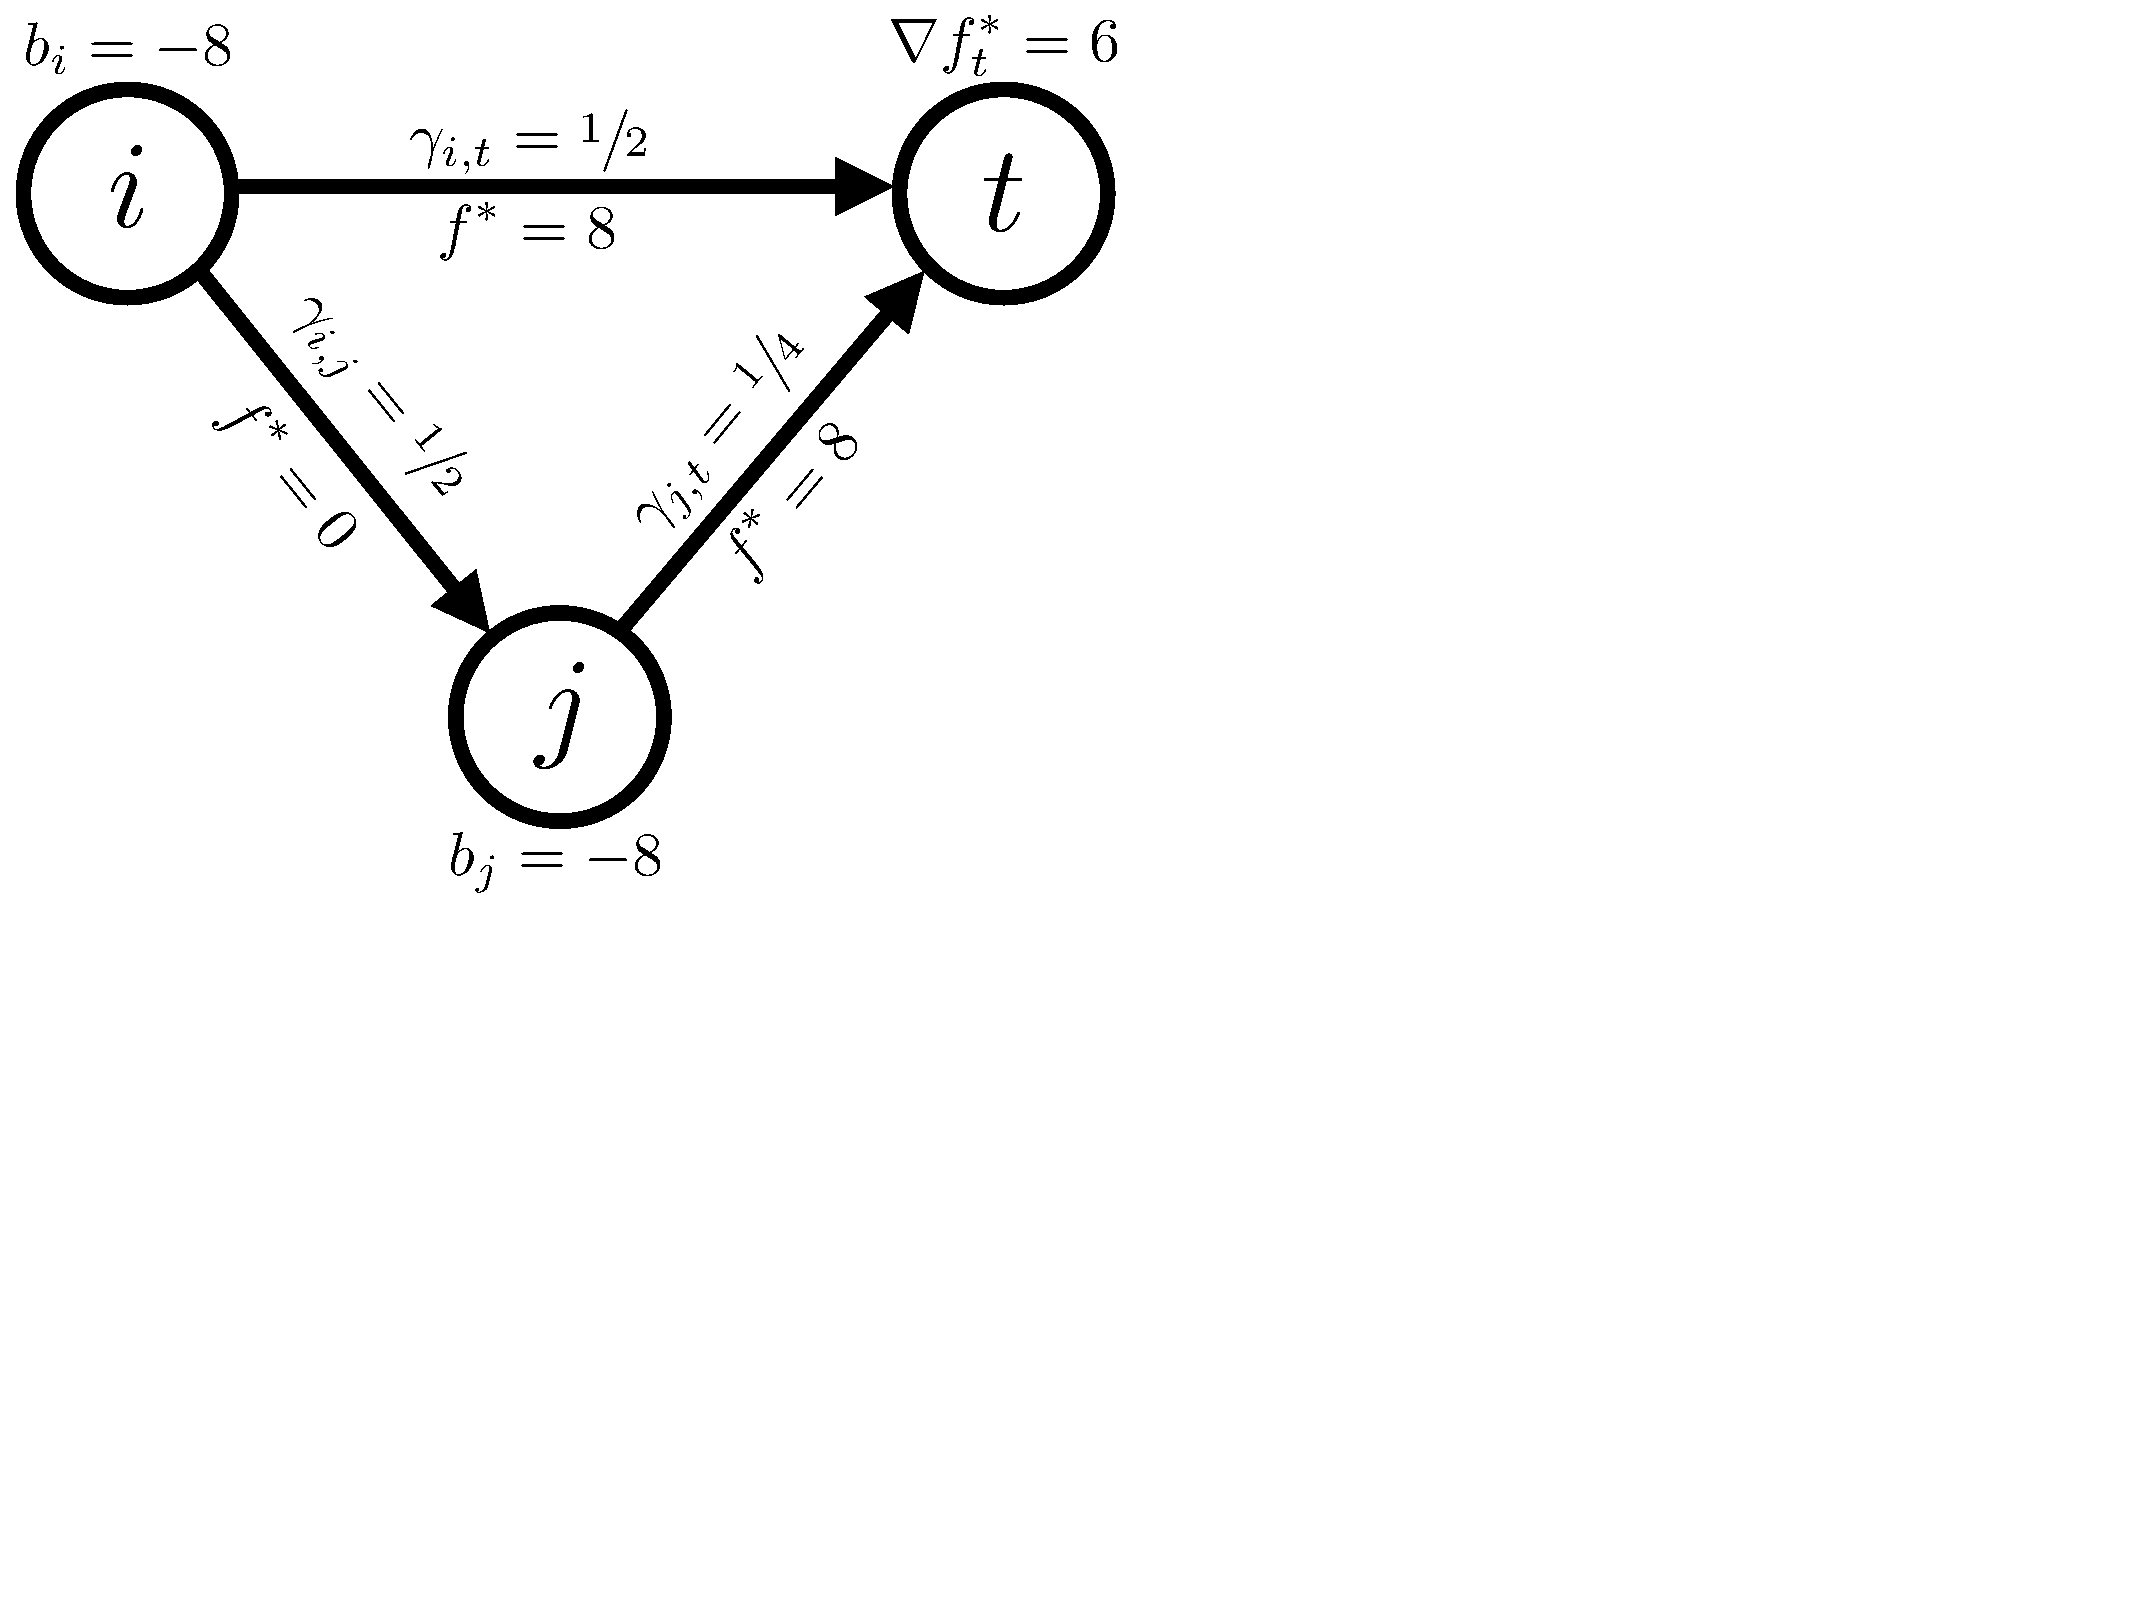
\includegraphics[width=0.8\linewidth]{figs/tight}
	\end{minipage}
	\begin{minipage}{.49\textwidth}
		\centering
		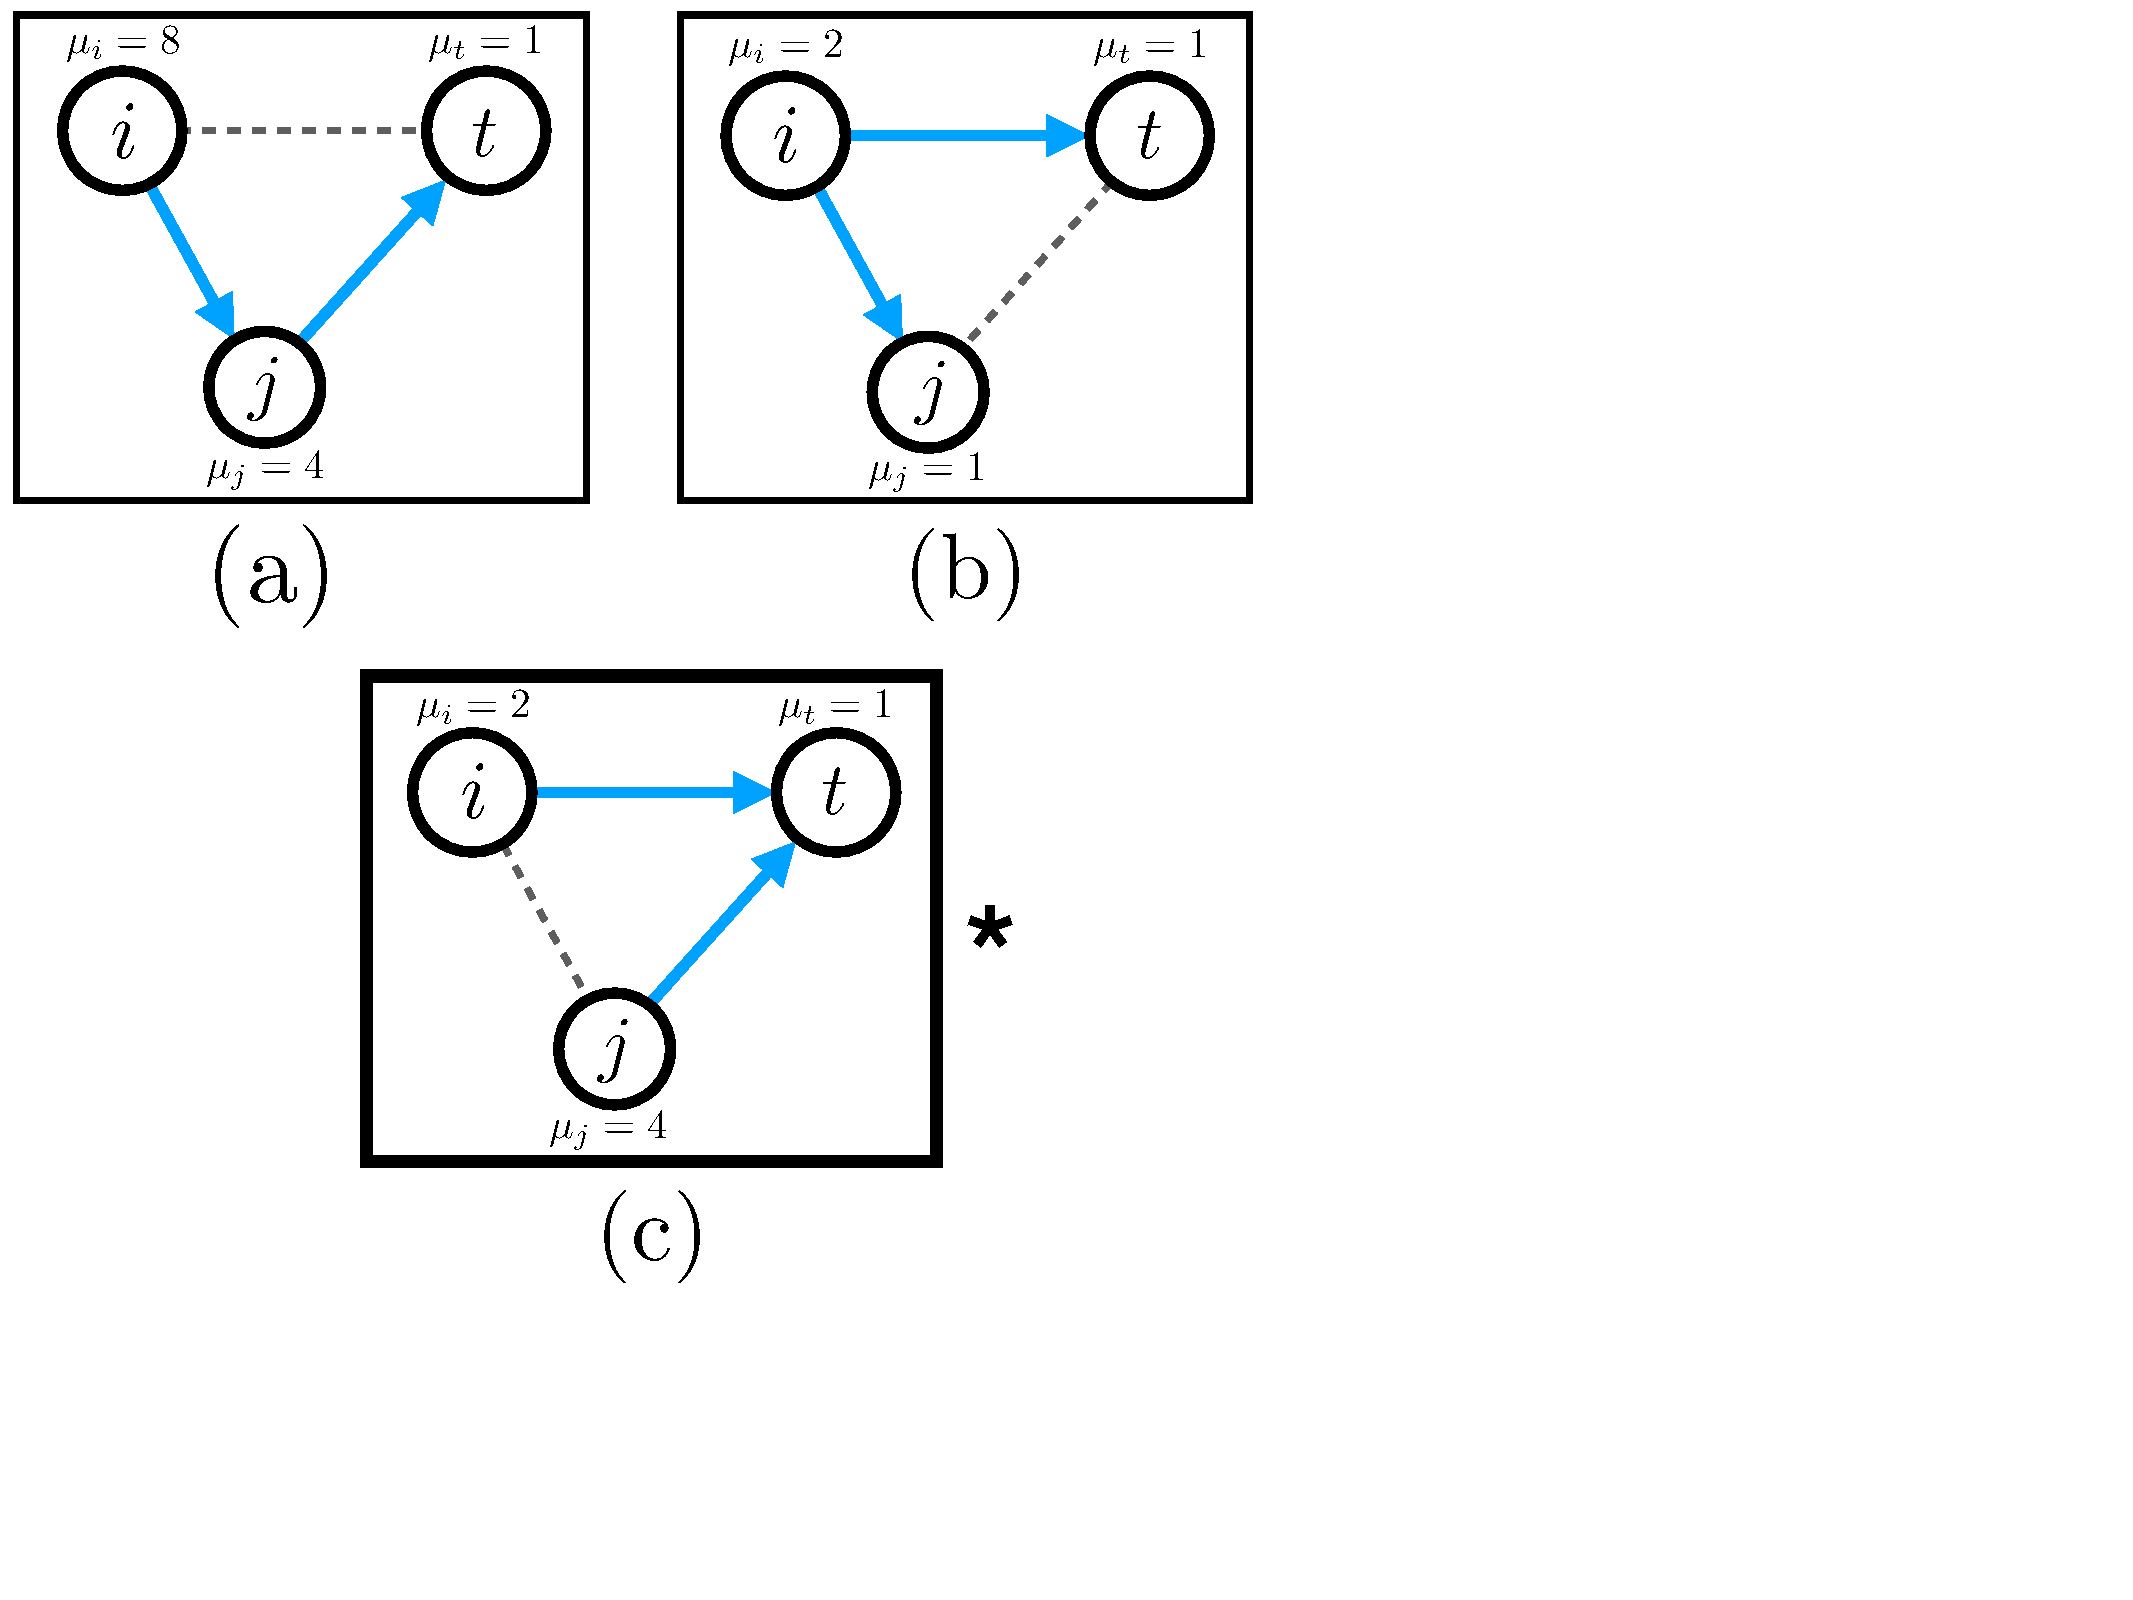
\includegraphics[width=.75\linewidth]{figs/tight-span-2}
	\end{minipage}
	\label{fig:ex-spanning}
	\caption{(left) Example flow network. (right) All three possible 
	spanning trees of tight edges and their respective dual solutions.
	Blue edges are tight ($\gamma^{\mu} = 1$), gray dashed edges are not.}
	\end{figure*}
	\end{example}
	
	
	\subsection{Contractibility Certificates} \label{sec:cert-contract}
	%Following from the previous two sections, in order to optimize the dual,
	%both algorithms make progress by alternating between finding contractible
	%edges and contracting them.
	The heart of both strongly polynomial algorithms detailed below is a procedure for
	identifying contractible edges and then contracting them.
	The key differences between the two algorithms are in 
	\textit{how} they find contractible edges, which
	we will describe in Sections~\ref{sec:2013} and~\ref{sec:2017}. These differences
	allow Olver and Végh \cite{Olver2017} to achieve a better running time bound than
	Végh \cite{Vegh2013}. The algorithms have in common the use of primal-dual pairs
	as certificates for contractibility.

	From Section~\ref{sec:motivate-dual}, complementary slackness tells us that if there is a primal optimal flow
	$f$ with positive value
	on some edge $e$, then $e$ is tight with respect to \emph{every} dual
	optimal solution---that
	is, $e$ is contractible. So a primal optimal flow provides a certificate
	for contractibility.
	It would seem this is of no use to us, as computing a primal optimal flow is the entire
	problem we are trying to solve. However,
	an optimal flow is a vastly superfluous certificate.
	
	Suppose instead that we have any flow $g$ and a bound on the difference
	between $g$ and an optimal
	flow $g^*$. Then if $g$ had a sufficiently large value on some edge $e$, we would know that
	$g^*_e > 0$. This idea is formalized in the following lemma, adapted from Lemma 3.3 of
	\cite{Olver2017}.
	
  	\begin{definition} \label{def:conservative}
  	Let $f$ be a feasible solution to (P).
	$\mu$ is a \textbf{conservative labeling} for $f$ if $\mu$ is
	a feasible solution to (D) and all edges with positive flow are tight. In this case,
	$(f, \mu)$ is called a \textbf{conservative pair}.
	\end{definition}

	\begin{lemma} \label{lem.bound-dist}
	Suppose $(g, \mu)$ is a conservative pair. Then there is some optimal flow $g^*$
    uniformly ``close'' to $g$:
    \[ \|(g^*)^\mu - g^\mu\|_\infty \leq \Ex(g, \mu). \]
    \end{lemma}
    \begin{proof}
    The intuition is that the optimal flow improves on the feasible flow by
    sending more of its excess to the sink. Thus, the difference $g^* - g$
    is a flow of value at most $\Ex(g, \mu)$ at $t$. The maximum edge value of
    the difference is bounded, in turn, by its total flow value.
    
	Since we are working with generalized flows, it will take a little work to formalize
	this idea. First, among all the optimal solutions to (P), let $g^*$ be the one
	which minimizes the total ($L^1$) difference $\|g^* - g\|_1$. Let $\mu^*$ be an
	optimal solution to (D). Then $(g^*, \mu^*)$ are a conservative pair---this is precisely
	the complementary slackness condition they satisfy.
	
	Let $h = g^* - g$. That is,
	\[ h_{ij} \coloneqq \begin{cases}
							g^*_{ij} - g_{ij} & \text{if } (i, j) \in E, \,
														   g^*_{ij} > g_{ij} \\
							\gij(g_{ij} - g^*_{ij}) & \text{if } (j, i) \in E, \,
																 g_{ji} > g^*_{ji}
						\end{cases} \]
    Observe that if $h_{ij} > 0$, then either $(i, j) \in E$ and $g^*_{ij} > 0$ or
    $(j, i) \in E$ and $g_{ji} > 0$. In other words,
    $(i, j) \in E_g$ and $(j, i) \in E_{g^*}$.
    
    \begin{claim} \label{claim:nocycles} $h$ is acyclic. \end{claim}
    \begin{proof}[Proof of Claim]
    Suppose that $h$ contains a cycle $C$. Then consider the net gain around $C$:
    \[ 1 \geq \gamma^\mu(C) = \gamma(C) = \gamma^{\mu^*}(C) \geq 1, \]
    as $\gamma^\mu \leq 1$ on $E_g$ and $\gamma^{\mu^*} \leq 1$ on $E_{g^*}$.
    As $\gamma(C) = 1$, we can slightly modify $g^*$ over the whole cycle to
    decrease $\|h\|_1$, contradicting the assumption on $g^*$.
    \end{proof}
    
    Now $h$ may be decomposed into a set of paths. Because $h$ is supported in $E_g$ and
    $\gamma^\mu \leq 1$ on $E_g$, flow can only decrease along these paths.
    As such, the total flow along any edge is at most the total flow leaving nodes:
    \[ \|h^\mu\|_\infty \leq \sum_i \max\,\{0, -\nabla h_i^\mu\}
     = \sum_i \max\,\{0, \nabla g_i^\mu - \nabla (g^*)_i^\mu\}
     \leq \sum_i \max\,\{0, \nabla g_i^\mu - \biu \}, \]
     which is $\Ex(g, \mu)$ as desired.
    \end{proof}
    The lemma suggests a concrete certificate for contractibility. An edge $e$ is
    \textbf{abundant} with respect to a conservative pair $(f, \mu)$
    if $f^\mu_e > \Ex(f, \mu)$.
    Lemma \ref{lem.bound-dist} shows that abundant edges are contractible.
    
    The contractibility certificate developed above determines the broad outlines
    for any contraction-based generalized flow algorithm. The algorithm's objective
    is to increase the maximum edge flow while keeping the total excess bounded.
    In order to achieve this, it will have to increase the demand values. Thus, the algorithm
    will consist of alternating \emph{scaling} and \emph{augmentation} phases.
    In the scaling phases, the dual variables $\mu$ are adjusted so that
    the values $|\biu|$ will increase. In the complementary augmentation phases,
    the algorithm spreads excesses around to keep them small.
		\frank{This is talking only about the 2013 one, not about both, and says
		"the"}
    
    Since the dual scaling will be a node-wise operation, it is more convenient
		in both algorithms
    to use a node-wise certificate of contractibility than the edge-wise one described
		above.\frank{Centralize definition of plentiful node here?}
    

\section{The Initial Strongly Polynomial Algorithm}
\label{sec:2013}
	%\subsection{Introduced Concepts and Notation}
    \label{sec:2013-notation}

%Notes for "Intuitive Section 4":

%-continuous scaling -> find contractible edges -> optimal dual -> optimal primal
%-continuous scaling -> breaks down usual $\Delta$ phases so won't over-shoot labeling
%-maintain feasible primal solution by keeping $\Delta$-feasible pair -- ensures security reserve $e_i >= R_i$
%-maintain bound on excess for individual nodes
%-trying to minimize max excess -- why?
%-push flow/excess around to create/identify abundant arc $(f_ij) >= 17m\Delta$
%-nodes with relabeled b magnitude $>= 20mn\Delta$ must have abundant arc adjacent
%-Pushes excess around by augmenting and relabeling; if algorithm gets "stuck", uses filtration to push flow around and even out excess in an "isolated" part of graph (not part of frontier)
%-algorithm maintains that b/delta is non-decreasing
%-cycle canceling only once in beginning -- explain why and assumptions?



A high-level overview of Végh's initial algorithm \cite{Vegh2013}
is shown below. This algorithm is characterized by a scaling factor $\Delta$,
which controls the amount of flow that can be augmented at each iteration and the threshold for
determining which edges are contractible. Sections \ref{sec:findconserv2013} and
\ref{sec:findcontr2013} expand on the details and provide intuition.
Section~\ref{sec:runtime2013} sketches the runtime
analysis of the algorithm, showing how it achieves a strongly polynomial bound.

\begin{enumerate}[(1),itemsep=0mm]
\item Find an initial feasible flow $\bar{f}$ and set initial $\Delta$ to
	  %$\max_{i \in V\setminus T} \nfiu - \biu$
	  the max relabeled excess of any node.
\item Compute an initial conservative labeling, $\mu$.
\item \label{step:2013-contract} Find contractible edges and contract until stopping condition is met
	(\emph{cf.} Section~\ref{sec:motivate-dual}).\\
	Contractible edges are found
	by repeatedly applying one of the following operations:
	\begin{enumerate}
		\item \label{step:2013-augment} Augment $\Delta$ units of flow.
		\item \label{step:2013-scale} Increase $\mu$ and decrease $\Delta$ by a factor $\alpha > 1$.
		\item \label{step:2013-filtration} Send flow from isolated parts of the graph directly to the sink.
	\end{enumerate}
\item Expand and find optimal primal solution via traditional max flow (\ref{sec:motivate-dual}).
\end{enumerate}

%\begin{definition}
%	For $\Delta \geq 0$, the \textbf{$\Delta$-fat graph} consists of all
%	forward edges $(i, j)$ and those reverse edges $(j, i)$ with $f_{ij}^\mu > \Delta$.
 %   \end{definition}

\subsection{Finding and Maintaining Conservative Pairs}
\label{sec:findconserv2013}
Following from primal-dual slackness, the optimality conditions for the primal
are (i) $\nfiu - \biu = 0$ for all $i \in \vnott$ and (ii) $\giij = 1$ if
$f_{ij} > 0$. The first condition is achieved by slowly reducing an upper bound
on the excess at each node as the algorithm continues. The second condition is
achieved by starting with an initial conservative pair (Definition~\ref{def:conservative})
and maintaining throughout the algorithm.

To find an initial conservative pair $(f,\mu)$, we must find a feasible flow
$\bar{f}$, calculate the initial labels using $\mu_t
\coloneqq 1$, and run a max flow to \rewrite{modify $\bar{f}$ with respect to $\mu$.}
\question{What does it mean to modify it with respect to u?}
$\bar{f} \equiv 0$ is a trivial
feasible solution to the capacitated version of the primal; this can be used to find an initial feasible solution for the uncapacitated representation by
following the transformation in \cite{article} (this just requires
adding a few additional edges and nodes). Once we have an initial conservative pair, we set the starting value of $\Delta$ equal to
$\max_{i \in V\setminus T} \nfiu - \biu$, which is the maximum relabeled excess
for any node (excluding $t$). This value is chosen because $\Delta$ controls the
amount of flow augmented at each iteration, and it wouldn't be feasible to send
more flow along a path than the maximum excess. Since $\Delta$ is monotonically
decreasing in the algorithm, we initialize it to the maximum feasible value.

The algorithm maintains a relaxed \textbf{$\Delta$-conservative pair},
which allows small amounts of flow (less than $\Delta$ units) along non-tight
edges.
%That is, it allows small (less than $\Delta$) flows along non-tight edges.
%\katie{why?}
The excess at each node is required to be at least the amount of incoming flow along non-tight edges. Thus, at any time, the flow can be made conservative (while remaining feasible) by zeroing flow along non-tight edges.
% The algorithm also maintains a uniform upper bound on excess,
% $\nfiu - \biu \leq 4(d_i + 2)\Delta$.
As $\Delta$ decreases, the amount of flow on these non-tight
edges decreases.

\subsection{Identifying Contractible Edges}
\label{sec:findcontr2013}
As discussed in Section \ref{sec:motivate-dual},
the algorithm makes progress by finding contractible edges.
As discussed in Section \ref{sec:cert-contract}, an edge is guaranteed
to be contractible when it is abundant. The algorithm maintains a pair $(f, \mu)$ with
a uniform bound on the excess $\nfiu - \biu \leq (4d_i + 8)\Delta$, whence
\question{What is whence supposed to mean here? Might be clearer to use a different word}
$\Ex(f, \mu) \leq 16m\Delta$.
Thus, an edge $(i, j)$ with $f_{ij}^\mu \geq 17m\Delta$ is abundant.
However, it is simpler to keep track of a certificate which depends only
on the dual variables $\mu$ as the flow $f$ changes:
\begin{claim}
If a node $i$ has $\abs{b_i^\mu} \geq 20nm\Delta$, then it must
have a contractible edge adjacent to it.
\end{claim}
\begin{proof}
Suppose by way of contradiction that none of the edges adjacent to $i$ are
contractible; this means that each edge $e$ must have $f_e^\mu < 17m\Delta$.
Consider the two cases below and note that $m \geq n \geq d_i + 1$ (\ref{sec:notation}).
\begin{enumerate}[itemsep=0mm]
\item First suppose $b_i^\mu > 0$. Then we obtain a contradiction to the feasibility of $f$:
      \[ \nfiu - \biu = \sum_{j \in \din(i)} \gamma_{ji}^\mu f_{ji}^\mu -
	  \sum_{j \in \dout(i)} f_{ij}^\mu - b_i^\mu < 17d_im\Delta - 20nm\Delta < 0. \]
\item On the other hand, if $b_i^\mu < 0$, then we obtain a contradiction to the
      bound $\nfiu - \biu \leq (4d_i + 8)\Delta$:
	  \[ \nfiu - \biu = \sum_{j \in \din(i)} \gamma_{ji}^\mu f_{ji}^\mu -
		 \sum_{j \in \dout(i)} f_{ij}^\mu - b_i^\mu
         > -17d_im\Delta + 20nm\Delta \geq 3nm\Delta + 17m\Delta. \qedhere \]
\end{enumerate}
\end{proof}

The algorithm maintains several sets of nodes. 
Let $L$ be the set of ``low excess'' nodes with $\nfiu - \biu < (d_i +1)\Delta$.
Let $H$ be the set of ``high excess'' nodes. A node enters $H$ when its excess hits the upper bound
$4(d_i + 2)\Delta$, and it stays in $H$ until its excess falls below $(d_i + 2)\Delta$. 
These bounds are illustrated in Figure~\ref{fig:lh}.
\begin{figure}[h!]
\centering
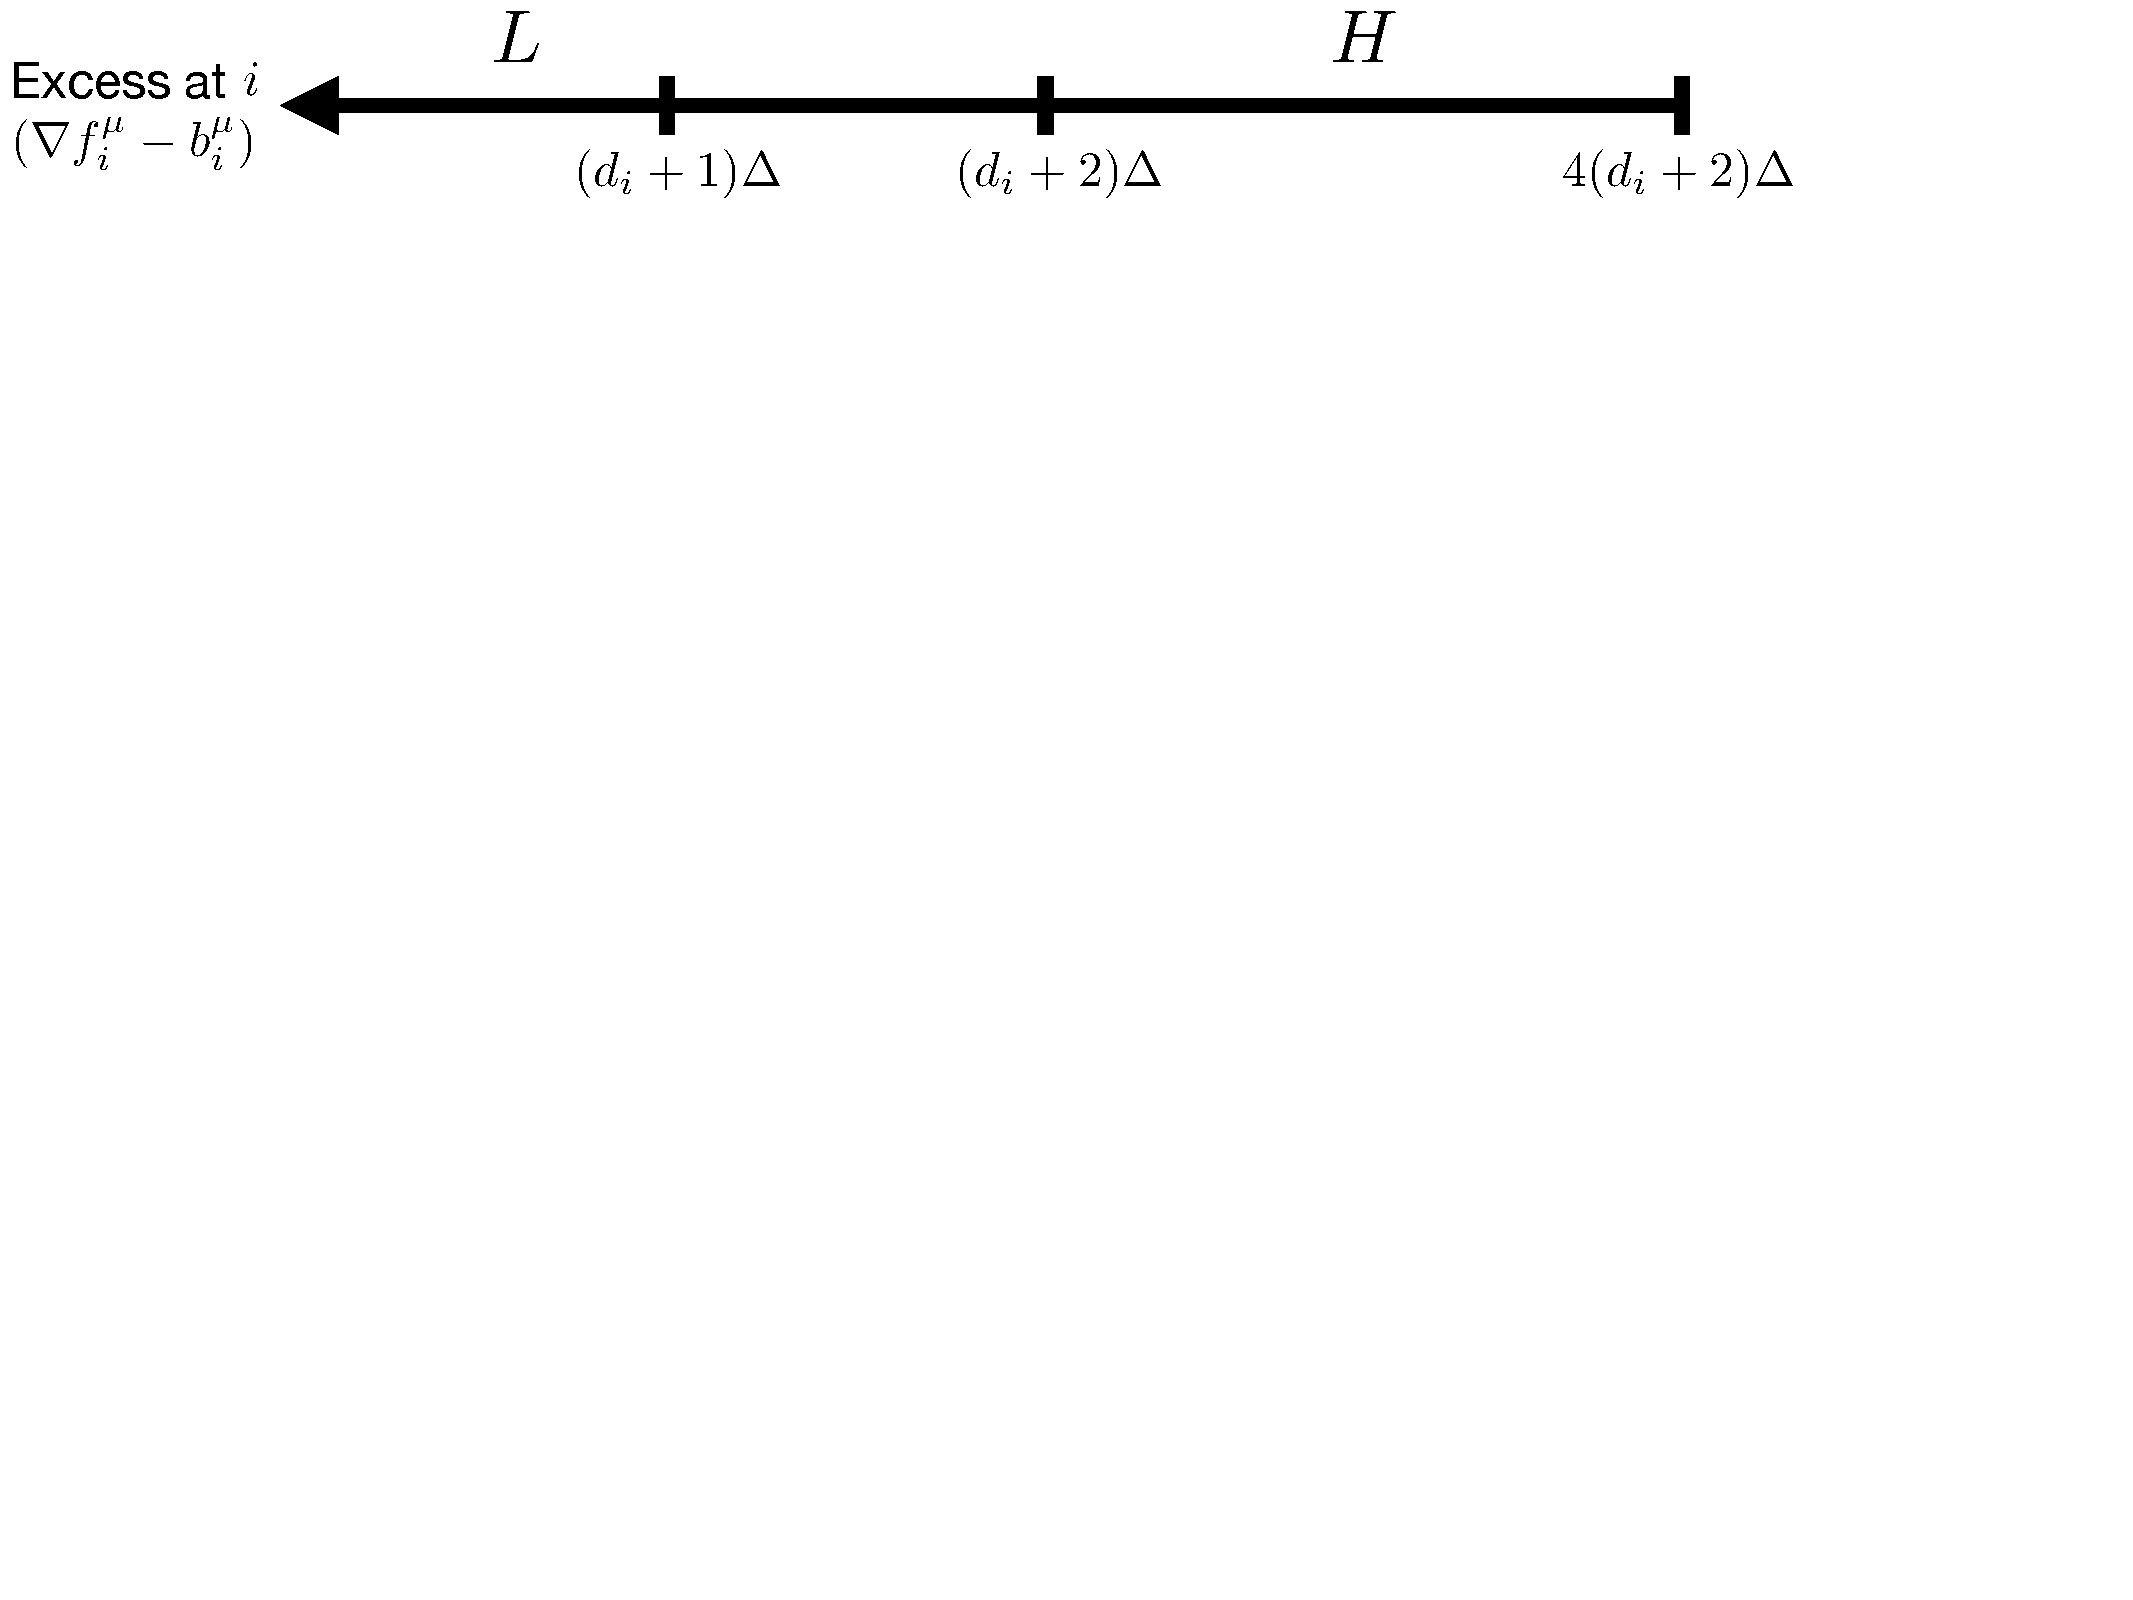
\includegraphics[width=\textwidth]{figs/lh.pdf}
\caption{
\label{fig:lh}
Number line showing values of excess when node $i$ is in set $L$ or $H$.
(\textbf{Not to scale}.)
}
\end{figure}

Finally, let $R$ be the set of nodes reachable along tight paths from $H$ (which is a
superset of $H$). The algorithm generally
seeks to spread excess from $H$ to $L$ along tight paths:

\begin{itemize}
	\item \textbf{\ref{step:2013-augment} Augmentation:} Each iteration of
		step~\ref{step:2013-contract} first looks to augment $\Delta$ units of flow on
tight paths from $H$ to $R \cap L$. This redistributes excess in order to
improve the balance of excess across the graph. 
%After augmentation,
%$R$ is reset to $H$ and the next iteration begins. 
%If the algorithm is not able to augment, then
When the algorithm is no longer able to augment,
there must either be (i) no
reachable low excess nodes to augment to or (ii) no high excess nodes to push
flow from.
\item \textbf{\ref{step:2013-scale} Scaling:} The scaling phase resolves both potential problems by increasing $\mu$ in $R$ and
decreasing $\Delta$ by the same factor $\alpha > 1$. 
\begin{enumerate}[(i),itemsep=0mm]
\item Increasing $\mu$ in $R$ causes
$\gamma_{ij}^\mu$ to increase for edges from $R$
to $V \setminus R$. This can cause an edge crossing this cut to become tight, which may add a low excess node to the set of reachable nodes.
% $\alpha_1$ is chosen to be $min \{\frac{1}{\giij}: ij \in E[R, V \setminus R]\}$. Intuitively, we want to choose an $\alpha$ that will bring $\gamma_{ij} \frac{\mu_i}{\mu_j}$ as close to 1 as possible without going over 1.
\item Decreasing $\Delta$ decreases the threshold for entering $H$, which may
	allow more nodes to be considered high excess.
This can continue until some node has excess equal to the upper bound $4(d_i + 2)\Delta$.
\question{Why does it have to reach the upper bound to be added to $H$?}
\question{"This CAN continue" or "does continue"...?}
\end{enumerate}
\begin{claim}
	The ratio $\sfrac{\abs{b_i^\mu}}{\Delta}$ is non-decreasing during scaling
	(and not changed during any of the other phases).
\end{claim}
\begin{proof}
$\alpha > 1$ by construction. The ratio does not change for nodes in $R$ since both
both $\biu = b_i/\mu_i$
and $\Delta$ are divided by $\alpha$.
In $V \setminus R$, the ratio is multiplied by
$\alpha$ because only $\Delta$ is divided by $\alpha$. 
\end{proof}
\item \textbf{\ref{step:2013-filtration} De-isolation:} If $V \setminus R$ does not contain any
nodes with large values of $\sfrac{\abs{b_i^\mu}}{\Delta}$,
then scaling will be ineffective in producing a plentiful node.
As such, if $\sfrac{\abs{b_i^\mu}}{\Delta} < \sfrac{1}{n}$ for every node
in $V \setminus R$, we delay scaling and focus on pushing
%redistributing the excess in $V \setminus R$.
%We compute a modified max flow along tight edges in $V \setminus R$.
%The goal is to push
flow directly to the sink from ``isolated''
nodes (i.e. those that are not reachable along a tight path from $H$).
The subroutine computes a modified max flow along tight edges in $V \setminus R$,
which
%The computed max flow values
replaces the current flow on edges
inside $V \setminus R$; flow on edges going from $V \setminus R$ to $R$ is zeroed,
and all other values remain the same. Reducing excess of nodes in
$V \setminus R$ might allow the next scaling phase to last longer and
thus increase $\sfrac{\abs{\biu}}{\Delta}$ more.
Simultaneously, zeroing the flow from $V\setminus R$ to $R$
reduces the excess of nodes in $R$, which might open them up to accept augmentations
in a future iteration.
\end{itemize}
% Scaling is the only phase of the algorithm that changes the important ratio
% \katie{why is it important?}
% $\sfrac{\abs{b_i^\mu}}{\Delta}$.

% Since this ratio is non-decreasing, the algorithm is always making progress towards finding a
% contractible edge; \rewrite{however, this progress might be very slow if the nodes that
% are increased in set $V \setminus R$ have small $\sfrac{\abs{b_i^\mu}}{\Delta}$
% values. In other words, investing time into the scaling phase in this scenario 
% yields small returns. To speed the process up, the algorithm prioritizes increasing the
% $\sfrac{\abs{b_i^\mu}}{\Delta}$ ratio for nodes that are already approaching the
% $20mn$ threshold; this progress is measured in comparison to $n$. We set a lower
% bound $\frac{1}{n}$ and add any node $i \in V-t$ with
% $\sfrac{\abs{b_i^\mu}}{\Delta} \geq \sfrac{1}{n}$ to $D$, which indicates
% these nodes are getting close to becoming abundant (i.e., they're worth investing
% in).} \katie{Do we ever say what happens to nodes in $D$? Otherwise, this paragraph could
% probably be cut too.}

% \frank{Currently trying to move this}
% \rewrite{
% If there are no augmentations to be made on a certain iteration, $\es$ is called
% if $D \cap V\setminus R \neq \varnothing$. 
% Since $\es$ only increases
% $\sfrac{\abs{b_i^\mu}}{\Delta}$ for nodes in $V\setminus R$, the subroutine will
% only be called if that set contains nodes that are close to reaching $20mn$. If
% there are no such nodes, a different subroutine, $\filtration$, is called first. 
% }

% \tocut{think we can cut most if not all of this}
% \rewrite{This alternation between augmenting, rescaling, and pushing flow from
% $V \setminus R$ to $t$ continues until the graph is contracted into one node.
% The optimal solution, $\mu$, to the contracted instance of the dual can then be
% easily extended to the original instance. This function essentially
% reverses the contraction operations by assigning a $\mu'$ value to the
% non-representative node (i.e. if edge $(p,q)$ was contracted and $p$ remained in the
% graph, assign $\mu'$ to $q$). The assigned $\mu'$ value is $\mu_p\gamma_{pq}$ if
% $p=t$ or $\frac{\mu_q}{\gamma_{pq}}$ if $p \neq t$. A final max flow is then run
% on the resulting optimal dual solution to get an optimal primal solution
% (Section~\ref{sec:motivate-dual}).}

\subsection{Sketch of Runtime Analysis} \label{sec:runtime2013}
In this section we analyze a few key ideas that lead to a strongly polynomial
runtime. The full (and lengthy) set of proofs for the runtime analysis can be
found in \cite{article}.

%For analysis, we divide these iterations into the following categories:

%\begin{enumerate}[(1),itemsep=0mm]
%	\item Shrinking Iteration: set R decreases by at least one node 
 %   	\begin{enumerate}
%    	\item Augmentation shrinks R because R is reset to H
%        \item $\es$ causes node's excess to decrease below H threshold and node becomes unreachable on tight path from H (i.e. no longer in set R)
 %   	\end{enumerate}
 %   \item Expanding Iteration: set R increases by at least one node
 %   	\begin{enumerate}
 %   	\item 
 %   	\end{enumerate}
 %   \item Neutral Iteration: Neither shrinking or expanding
%\end{enumerate}

As noted in Section \ref{sec:motivate-dual}, there can only be $n-1$ contractions. Therefore
the analysis aims to show a contractible edge can be found in strongly polynomial time.
We define the following potential function to bound the number of iterations of
step~\ref{step:2013-contract} defined at the beginning of Section~\ref{sec:2013}.
\[ \Psi \coloneqq \sum_{i \in H} \left\lfloor \frac{\nfiu - \biu}{\Delta} - (d_i + 1) \right\rfloor \]

Recall that $H$ denotes the set of ``high excess'' nodes.
The potential increases by $4(d_i + 2) - (d_i + 1) = 3d_i + 7$ when a node is
added to $H$ (this is called an \textit{expanding iteration})
and decreases by $(d_i + 2) - (d_i + 1) = 1$
when a node leaves $H$ (a \textit{shrinking iteration}). Once a node leaves
$H$, $\Delta$ must decrease by at least a factor of two before that node can enter $H$ again; this allows us to
bound the total number of expanding iterations. Since $H$ is initially empty
($\Psi = 0$), we can use the bound on expanding iterations to bound the total increase in
potential. Furthermore, since a node in $H$ must have $\nfiu - \biu \geq \Delta(d_i + 2)$,
$\Psi$ is always nonnegative. This allows us to use the
total increase in potential to bound the total decrease in potential, and, in turn,
the number of shrinking iterations.

\question{This entire paragraph doesn't make much sense, most likely because those two things aren't defined anywhere}
This gives us strongly polynomial bounds on the number of expanding and
shrinking iterations; however, we must also prove that there are only a few
\textit{neutral} iterations in between these expanding and shrinking iterations.
This is where we note the importance of the set $D$ and the $\filtration$
subroutine. On each iteration, if there is not an augmentation (shrinking), then
either $\es$ or $\filtration$ and $\es$ will be called. If $\es$ is called, then
this means set $V \setminus R$ has at least one node in $D$ that will have its
$\sfrac{\abs{b_i^\mu}}{\Delta}$ increased by $\alpha$. Since this node is in D,
its $\sfrac{\abs{b_i^\mu}}{\Delta}$ value is at least $\sfrac{1}{n}$, which means
it will become abundant in a strongly polynomial number of iterations. If
$\filtration$ is called first, then the excess of nodes in set $V \setminus R$
will decrease enough such that $\es$ will cause one of these nodes to enter set
$D$ or these low excess nodes will enter set $R$, allowing an augmentation
(shrinking iteration) on the next iteration. Note the first option can only
happen $n-1$ times because once a node enters $D$, it cannot leave
($\sfrac{\abs{b_i^\mu}}{\Delta}$ is non-decreasing) unless it is contracted.
\katie{$D$ and $\es$ need to be defined somewhere above}
The analysis above gives us a strongly polynomial bound on the total number of iterations.
The maximum flow computation in $\filtration$ dominates the runtime per iteration.
This gives a total runtime of $O(n^3m^2\log n)$ (all other operations including initialization
are dominated by this runtime).
\question{Where does this runtime come from?}

%This algorithm achieves a strongly polynomial runtime by improving upon scaling techniques used in previous weakly polynomial algorithms such as FAT-PATH \cite{Goldberg:1991:CAG:105014.105022} and also by integrating the concepts of abundant and contractible edges from Orlin's minimum cost flow algorithm \cite{Orlin1988}. 

%Orlin's \textit{abundant arc} concept can be applied to generalized max flow to show that if an edge has a large amount of flow in comparison to the value of the scaling factor $\Delta$, then that edge must have non-zero flow in the primal solution and, by complementary slackness, the edge must be tight in every dual solution. Therefore that edge can be contracted as shown in Section~\ref{sec:contract}. At a high-level, Végh's generalized max flow algorithm maintains a feasible primal solution while trying to identify these contractible edges to find an optimal dual solution. Once found, the optimal dual solution can be used to easily transform the feasible primal solution to an optimal primal solution via one traditional max flow iteration as shown in Section~\ref{sec:motivate-dual}.

%In order to find contractible edges in strongly polynomial time, this algorithm introduces the concept of \textit{continuous scaling}. Previous scaling algorithms for this problem use distinct $\Delta$-scaling phases, where $\Delta$ is only updated after a constant number of path augmentations. This can cause an ``over-shooting'' problem in which $\Delta$ increases too quickly relative to $f^\mu$ to guarantee abundant edges. As a solution, this algorithm continuously alternates between augmenting $\Delta$ units of flow from ``high-excess'' nodes to ``low-excess'' nodes (including the sink) and proportionately increasing $\mu$ and decreasing $\Delta$. Since $\Delta$ and $\mu$ are always scaled coherently, their relative magnitude stays bounded and non-decreasing, which addresses the over-shooting problem.
%\label{sec:2013}
	
	%This algorithm employs scaling parametrized by a factor $\Delta$.
    
   % Végh's initial strongly polynomial algorithm \cite{Vegh2013}
%	introduces the notion of a \textit{conservative labeling}, which helps to
%	identify the highest gain augmenting paths on which to push flow.
%	\begin{definition}
%	$\mu$ is a \textbf{conservative labeling} for $f$, a feasible solution to (P), if $\mu$ is
%	a feasible solution to (D) and all edges with positive flow are tight.
%	\end{definition}
 %   \begin{definition}
 %   $\mu$ is a $\Delta$-conservative labeling for $f$, or alternatively $(f, \mu)$ are a
%	$\Delta$-feasible pair, if
  %      \begin{enumerate}[(i)]
 %       \item $f_{ij}^\mu \leq \Delta$ for all non-tight edges $(i, j)$;
 %       \item $\mu_t = 1$; and
 %       \item $\mu_i > 0, \nfi - b_i \geq R_i$ for all $i \in V \setminus t$ where $R_i$ is the total incoming flow on non-tight edges
  %      \end{enumerate}
  % \end{definition}
    
%	The scaling algorithm aims to identify \emph{contractible} edges,
	%edges that are tight in every optimal dual solution,
  %  in a strongly polynomial number of steps. This technique was
  %  originally developed to study the minimum cost flow problem (\emph{cf.}~\cite{Orlin1988}). \todo{need to define this or refer to section 3?}
%	As we will show in Section~\ref{sec:infeasible} Lemma~\ref{lem.contractibility}, a large flow value along an edge can
 %   serve as a certificate of contractibility. To that end, we define
 %   \begin{definition}
 %   An edge $(i, j)$ is \textbf{abundant} at scale $\Delta$ if $f_{ij}^\mu \geq 17m\Delta$.
  %  \end{definition}
%		\todo{At least give intuition for how they derived this number}
%	Once the algorithm identifies an abundant edge,
%	it can contract the edge and reduce the size of the graph. The algorithm
%	terminates once the graph reduces to one node; this leads to a
%	strongly polynomial bound on the number of iterations of this algorithm.

%This algorithm also extends the scaling technique in the FAT-PATH algorithm
 %   \cite{Goldberg:1991:CAG:105014.105022} by introducing \textit{continuous scaling}. At a high-level, the continuous scaling
 %   method alternately (i) augments $\Delta$ units of flow along a tight path from high
 %   excess nodes to low excess nodes (including the sink) or (ii) proportionately increases $\mu$ and
  %  decreases $\Delta$. Unlike previous scaling methods used for the generalized flow problem, such as FAT-PATH \cite{Goldberg:1991:CAG:105014.105022},
 %   this algorithm does not have distinct $\Delta$-phases; instead, $\Delta$ is updated continuously.
    
  %  As $\Delta$ and $\mu$ are always scaled coherently, their relative magnitude will stay bounded.
 %   This addresses an ``over-shooting'' problem common in previous scaling algorithms in which $\Delta$
 %   increases too quickly relative to $f^\mu$ to guarantee abundant edges.
    
 %   As $\Delta$ changes, the algorithm maintains a $\Delta$-feasible pair, which ensures that there is
  %  a ``reachable'' feasible solution to (P). If $(f,\mu)$ is a $\Delta$-feasible pair,
  %  setting the flow on non-tight edges to zero yields a feasible pair.
 %   Given this, the algorithm only needs to run a cycle-canceling
 %   algorithm once on the initial solution and then feasibility is maintained throughout the rest of
 %   the algorithm.
    
	%\subsection{Algorithm Overview} \label{sec:2013-overview}
	%\begin{table}[H]
	%\begin{center}
	%    \begin{tabular}{ | p{7cm} | p{7cm} |}
	%    \hline
	%    Challenges in Previous Algorithms  & Solutions from Algorithm \\ \hline
	%    ``Abundant edge'' might not appear in strongly polynomial number of steps \cite{Radzik2004} & Continuous Scaling Method  \\ \hline
	%    Augmentation along highest gain paths introduce flow generating cycles; must run cycle-canceling algorithms in every scaling phase \cite{Goldberg:1991:CAG:105014.105022} & Maintain a $\Delta$-conservative pair, which guarantees feasible solution to (P); only need to run cycle-canceling once in initialization  \\ \hline
	%    ``Inflation'' in scaling algorithms; labels increase too much causing relabeled flow to be $\ll \Delta$. A new abundant edge may never appear. & Continuous scaling and Filtration subroutine \\
	%    \hline
	%    \end{tabular}
%	\end{center}
%	\caption{Key Improvements On Previous Algorithms}
%	\label{tab:improvementsInitial}
%	\end{table}
	
   % The key ideas that lead to improvements in this algorithm, as compared to previous algorithms,
   % are summarized in Table~\ref{tab:improvementsInitial}.
    
  % This algorithm is the first strongly polynomial algorithm for generalized maximum flow and has a running time of $O(n^3 m^2 \log n)$. In this section, we give an overview of the algorithm. In Section \ref{sec:tf}, \ref{sec:es}, and \ref{sec:filtration} we further explain the three main functions called in the algorithm. %This algorithm can be extended to  however, the $\log n$ term can be reduced by performing extra bookkeeping on flow values from previous iterations. This is explained in detail along with proofs of polynomially-bounded number sizes in Végh's full version of the paper~\cite{article}.
	     
	%Given an initial feasible solution to (P), the algorithm first runs a cycle-canceling algorithm,
	%	which gives a conservative labeling $\mu$ in strongly polynomial
	%	time\todo{?}. The bulk of the
  %  work in the algorithm is spent identifying and contracting abundant edges. This continues
  %  until the graph is contracted to one node. Once an optimal solution, $\mu$, to (D)
 %   is found for the contracted graph, it can easily be transformed into an optimal solution to
 %   (D) for the original graph. This is done by reversing the contraction step (full details
 %   are given in \cite{article}). The optimal dual solution can then be converted into an optimal solution to (P) by running one max flow computation (\tf\ subroutine). %\tf\ is then run one last time to convert the
    %optimal dual solution into an optimal solution to (P).
	
	%While finding and contracting edges, the algorithm maintains several sets as defined below:
	%\begin{align*}
	%N&\text{: set containing sink and ``low relabeled excess'' nodes with }
  %          \nfiu - \biu < (d_i +1)\Delta \\
	%T_0&\text{: set of ``high relabeled excess'' nodes with } \nfiu - \biu \geq (d_i + 2)\Delta \\
	%T&\text{: set of nodes reachable on a tight path from $T_0$ in $\Delta$-fat graph} \\ 
%	D&\text{: set of nodes $i \in V \setminus t$ with } \abs{b_i^\mu} \geq \Delta / n
	%\end{align*}
	
	%On each iteration, the algorithm augments along a tight path if possible. Otherwise, if there
  %  are no tight paths between nodes of high excess and nodes of low excess, the algorithm checks
   % if there are tight paths connecting high excess nodes to nodes not included in sets $T$ or $N$;
   % if so, a node along this tight path is added to set $T$. If the algorithm cannot push flow
  %  or expand the ``frontier'', then \filtration is called to reduce the excess of relatively
  %  isolated nodes. This is useful because it expands the set of ``low excess'' nodes that flow
  %  can be pushed to, which allows augmentation. It is important to note that this last option
  %  can only be computed at most $n - 1$ times because once a node is in set $D$, it cannot leave.
  %  This is because the ratio $\abs{b_i^\mu} / \Delta$ is non-decreasing. Below is a high-level
  %  overview of the procedure used to find contractible edges:
   % \todo{Use algorithm package if time}
%	\begin{align*}
%	&\text{IF $N \cap T \neq \varnothing$} \\
%	&\quad \text{Push $\Delta$ units of relabeled flow along a tight path from $i \in N$ to $j \in T$} \\ 
%	&\quad \text{Update sets accordingly} \\
%	&\text{ELSE ($N \cap T = \varnothing$)} \\
%	&\quad \text{IF $\exists$ tight path from $i \in T$ to $j \in V \setminus T$} \\
	%&\quad \quad \text{Add node $j$ to $T$} \\
	%&\quad \text{ELSE} \\
	%&\quad \quad \text{IF $(V \setminus T) \cap D = \varnothing$} \\
	%&\quad \quad \quad \text{\filtration($V \setminus T$)} \\
	%&\quad \quad \text{\es($T$)} 
	%\end{align*}
	
	%At the end of each iteration, the algorithm checks if an abundant edge has been
   % identified (and if so, it is contracted) or if the termination condition has been met.
  %  Once this loop terminates, the graph is expanded and a final max flow computation
  %  is run to find the optimal solution to (P).
%	\subsection{\tf\ Subroutine}\label{sec:tf}
    
%	The \tf\ subroutine is used at initialization to find an initial feasible flow $f$ and at
 %   termination to convert the optimal dual solution to an optimal solution to (P).
 %   It is also used in the \filtration\ subroutine (Section~\ref{sec:filtration}).
 %   This algorithm is essentially a standard maximum flow computation on the input
 %   set and an added source node. If the max flow computation is infeasible (due to the
 %   negative upper bounds), then an error is returned. We present the main theorem
 %   given in \cite{Vegh2013} below and also transform their explanation of the
 %   subroutine into pseudocode for a more clear representation.
	%\begin{theorem}
	%If $\mu$ is an optimal solution to (D), then $\tf(V, \mu)$ returns an optimal solution to (P).
    %\todo{this theorem is verbatim from paper---another way to phrase it?}
	%\end{theorem}
	%\todo{proof?}

	%\begin{align*}
	%&\text{\textbf{Input:} Set $S \subseteq V$ with $t \in S$ and labeling $\mu$ that is
   %        dual-feasible everywhere in $S$---i.e., $\giij \leq 1$ for all $i, j \in S$} \\
%	&\text{\textbf{Output:} Flow $f'$ such that $(f', \mu)$ is a conservative labeling
  %         everywhere in $S$} \\
%	&\text{Add source node $s$ and edges $(s, i)$ for all $i \in S \setminus t$} \\
%	&\text{Set upper and lower bound capacities, $u$ and $l$, as follows: } \\
%	&\quad \text{For all tight edges $(i, j)$: $u_{ij} = \infty$ and $l_{ij} = 0$} \\
%	&\quad \text{For all edges $(s, i)$: $u_{si} = -\biu$ and $l_{si} = -\infty$} \\
%	&\text{Run max flow $x$ on node set $S \cup \{s\}$ and the set of tight edges} \\
%	&\text{Return $f'$ such that}
 %   \end{align*}
 %   \[ f'_{ij} = \begin{cases} x_{ij} \mu_i & \text{if edge } (i, j) \text{ is tight} \\
 %   					       f'_{ij}      & \text{otherwise}
 %                \end{cases}
  %  \]
	
%	\subsection{Elementary Step Subroutine}\label{sec:es}
    
	%In a scaling step, $\Delta$ is continuously scaled down
  %%  and $\mu_i$ scaled up for $i \in T$. The flow on edges from $V \setminus T$ to $T$ and the flow
  %  on non-tight edges contained in $V \setminus T$ are also scaled down. This continues as long
  %  as $(f, \mu)$ remains $\Delta$-feasible and as long as the excess for each node $i$
 %   remains bounded by a quantity proportional to $\Delta$ and $\mu_i$.
 %   Once all values have been rescaled, the sets $T$ and $T_0$ are modified accordingly.  
	
%	\subsection{Filtration}\label{sec:filtration}
    
%	The \filtration\ subroutine is used to ``clean up'' the set of nodes $V \setminus T$ if
 %   all of the nodes have a high amount of excess relative to their demands. 
  %  It reduces the relabeled excess of these nodes,
  %  which increases the number of
  %  ``low excess'' nodes to push flow to,
  %  and then runs \tf\ on $V\setminus T$,
  %  which returns a new flow $f'$. The flow values are modified as follows: 
	%\begin{itemize}[itemsep=-1mm]
%	\item Edges entering $T$: $f_{ij}$ = 0
%	\item Edges leaving $T$: no change
%	\item Edges contained in $T$: no change
%	\item Edges contained in $V\setminus T$: $f_{ij} = f'_{ij}$
%	\end{itemize}
	
%	If these modifications reduce the excess of a node $i$ enough to either remove $i$ from set $T_0$
 %   ($i$ is no longer a high excess node) or add $i$ to set $N \cap T$ ($i$ is now a reachable
  %  low excess node), then the algorithm terminates and the next iteration of the
  %  ``finding a contractible edge'' is performed. Otherwise, the algorithm terminates
  %  and the elementary step routine is called to relabel.

	%	\todo{Need to tie everything together somehow}
	%	\todo{Runtime analysis?}

\section{A Faster Strongly Polynomial Algorithm}\label{sec:2017}

The most recent strongly polynomial algorithm developed by Olver and Végh
\cite{Olver2017} takes the same overall approach as the original
algorithm~\cite{Vegh2013}, but introduces several novel ideas that improve the running time by a factor of almost $O(n^2)$. 
In this section, we describe the algorithm and provide intuition for the
improved running time.
 %A highlight of the difficulties in
%previous algorithms and the subsequent solutions from this algorithm are
%summarized in Table~\ref{tab:improvements}.

%\begin{table}[H]
%\begin{center}
%\begin{tabular}{ | p{7cm} | p{7cm} | p{2cm} | }
  %  \hline
%		Challenges in Previous Algorithms  & Solutions from New Algorithm & Why \\ \hline
 %   Non-integral flow values & Only store relabeled flow $f^{\mu}$ which stays
%		integral throughout the algorithm until the last step of computing optimum & \\ \hline
 %   Initial cycle-canceling algorithm to eliminate flow generating cycles & Two
%		phase method (similar to simplex) where feasible solution found in first
%		phase is used to start the second phase; this solution is faster than the
	%	cycle-canceling subroutine & \\ \hline
 %   Complex methods for maintaining feasible flow & Relax flow feasibility (node
%		demands do not have to be met) and use complementary slackness properties to
%		keep feasible primal solution "within reach" & \\ \hline
%    No guarantee of abundant edge appearing in strongly polynomial number of
\iffalse		steps \cite{Radzik2004} &  Continuous scaling & \\ \hline
    Complicated multiplicative potential analysis \cite{Vegh2013} & Additive
		potential analysis & \\
    \hline
    \end{tabular}
\end{center}
\caption{Key Improvements of New Algorithm}
\label{tab:improvements}
\end{table}
\fi
	
	%%% TEMP %%% 
%%%	They want the set of tight edges, only at any given time actually have a dual solution. Only operations that happen to the edges are contractions or adding more tight edges, so tight edges never get removed. Inductive. The way to ensure tight edges never have to be removed is the safety property: ensure that their set of tight edges is always satisfiable, some flow that will only be supported on that set. Safety property can be maintained with the label update. 
	
%%%	Safety property is existence of a flow. Un-safety is equivalent to existence of Hoffman's property / cut. Scaling constructed so that it never breaks any of these sets. If there's a set that's violated in $\mu'$, then if you take the set excluding the parts that were modified then it must have already been violated. Modification only increased the values of $\biu$ inside $S$.
	
%%%	If there's a violated set, divided into two pieces, part in $S$, part not in $S$. One of them had to already be violated. Assume $\mu$ is safe and for the sake of contradiction that $\mu'$ is not safe. Then prove that if that were the case $\mu$ must have not been safe. 
%%%	$S$ is maximal subset that contains $Q$ and has no tight edges coming into it or out of it. Any modification done to $S$ is not going to change tight cuts because they must be either entirely inside or outside, not across the boundary, so scaled equally. 
	
%%%	Start with a feasible fitting flow. Find something close in $L_1$-norm (sum), decompose into paths to bound the difference between them. The difference between them is a flow and can't have any cycles because.
%%%	Important that $\mu$ be safe, because it assumes that there is a fitting pair and feasible $\mu$
%%%	If value of pseudoflow on edge is really high then optimal flow must have some flow on that edge becasue optimal flow has to be close enough to the pseudoflow
	
	%%% TEMP %%%
    
    %\label{sec:2017-intro}
%     As in the initial strongly polynomial generalized flow algorithm, this algorithm makes progress by
%     identifying contractible edges and then contracting them until a dual optimal
%     solution is found. Each contraction collapses one node, so only $n$ contractions
%     can occur. To identify and reason about contractible edges, we need a certificate
%     (sufficient condition) for contractibility. This is an elaboration of the \emph{abundant edge}
%     idea from Section \ref{sec:2013-notation}. \katie{could reduce this intro section since info already contained elsewhere}

	\subsection{Working with Infeasible Flows}\label{sec:infeasible}
	The algorithm described in Section \ref{sec:2013} maintains a feasible flow
	at all times. In order to produce a contractibility certificate, it has
	to keep the excess at each node bounded. In order to do that, it has to spread
	flow around, leveling out the excesses. In contrast, Olver and V\'egh \cite{Olver2017} maintain
	a possibly infeasible flow, introducing the possibility of deficit at a node. Excesses are sent to cancel with deficits instead of spreading them
	around. Whereas leveling excesses could require augmenting between all pairs of
	nodes (roughly $n^2$ pairs to consider), cancelling excess only requires identifying
	a corresponding deficit for each excess (roughly $O(n)$). This gives some intuition
    for why relaxing the feasibility requirement might be appealing.
	
	More precisely, the algorithm maintains a \textbf{fitting pair}
	of primal and dual solutions $(f,\mu)$. This is a relaxation of the idea of
	a conservative pair from Section \ref{sec:cert-contract}, wherein $f$ is not required
    to be feasible:
	\begin{definition}
	A (not necessarily feasible) flow $f$ is said to \textbf{fit} a feasible dual solution $\mu$
    if it satisfies the putative complementary slackness condition: $f_{ij} > 0 \implies \giij = 1$.
    In this case, we refer to $(f, \mu)$ as a \textbf{fitting pair}.
	\end{definition}
    
	In lieu of maintaining a feasible $f$ at each step,
	the algorithm ensures that $\mu$ is \textbf{safe}---i.e.,
    that a feasible $f$ fitting $\mu$ \emph{exists}---by preserving a
		cut property. To simplify the exposition, we start with a definition.
	\begin{definition}
		Recall that $\tau(\mu)$ denotes the set of tight edges under a dual labeling $\mu$.
		Given $\mu$, an \textbf{inward-loose cut} is a set $S \subseteq V$ that does
		not have any tight incoming edges 
		($\din(S) \cap \tau(\mu) = \varnothing$).
%         An \textbf{outward-loose cut}
% 		does not have any tight outgoing edges ($\dout(S) \cap \tau(\mu) = \varnothing$).
%         A \textbf{bi-loose cut} is both inward- and outward-loose.
	\end{definition}
	If $f$ is a flow fitting $\mu$, then there is no flow into inward-loose cuts because
	there are no tight edges to flow along.
	If $f$ is feasible, then it follows that the total demand inside an inward-loose
	cut is nonpositive---otherwise $f$ would have to satisfy this demand by flowing
	into the cut.
	It turns out that this is a sufficient condition for the existence
	of a feasible fitting flow:
	\begin{lemma}[Certificate for Safety] \label{lem.safety}
	$\mu$ is safe if and only if for any inward-loose cut $S \subseteq \vnott$,
	\[ \sum_{i \in S} \biu \leq 0. \]
	\end{lemma}
	This is a corollary of Hoffman's Circulation Theorem (\cite{Schrijver2002}, Theorem 11.2),
    a standard result on existence
    of (ordinary, not generalized) flows, applied to the tight graph under $\mu$.
% 	\begin{proof}
% 		Suppose the cut condition holds. Let $f$ be a flow on tight edges minimizing
% 		the total deficit $\Def(f, \mu) = \sum_i \min\{0, \biu - \nfiu\}$. Let
% 		$T^+$, $T^-$ be the sets of nodes with excess and deficit, respectively:
% 		\[
% 			T^+ = \{i \in V \mid \nfiu > \biu \} \qquad T^- = \{i \in V \mid \nfiu < \biu \}.
% 		\]
% 		Consider the residual graph of $f$ in the tight graph. If there were a path
% 		connecting $T^+$ to $T^-$, then we could augment along the path
% 		to reduce the total deficit. Therefore, there is no such path. Consider the
% 		set $T$ of nodes from which $T^-$ is reachable along tight edges (including reverse edges).
% 		The absence of a residual path from $T^+$ to $T^-$
%         implies that $T \cap T^+ = \varnothing$, whence
% 		\[ \sum_{i \in T} \nfiu - \biu = \sum_{i \in T^-} \nfiu - \biu < 0. \]
% 		By definition, $T$ is inward-loose. Therefore, the total flow into $T$ is zero.
%         Moreover, the total flow out of $T$ is zero, for otherwise there would be
%         residual tight edges into $T$. So
% 		\[ 0 = \sum_{e \in \din(T)} f_e - \sum_{e \in \dout(T)} f_e
% 		     = \sum_{i \in T} \nfiu < \sum_{i \in T} \biu, \]
% 		contradicting our assumption. It follows that $T^- = \varnothing$, i.e., $f$
% 		is feasible.
% 	\end{proof}
    
    \subsection{A Refined Contractibility Certificate}\label{sec:contract-cert}
    So long as the algorithm maintains the safety of $\mu$,
    we can obtain a feasible fitting flow $f$ at any time
    by running an ordinary maximum flow algorithm restricted to the tight graph of $\mu$.
    Moreover, a generalization of Lemma \ref{lem.bound-dist} applies to fitting
    pairs.
    \begin{lemma} \label{lem.bound-dist1.5}
    Suppose $(g, \mu)$ is a fitting pair with $\mu$ safe. Then there is some feasible flow $\tilde{g}$
    uniformly ``close'' to $g$:
    \[ \|\tilde{g}^\mu - g^\mu\|_\infty \leq \Def(g, \mu) \quad \text{and} \quad
       \Ex(\tilde{g}, \mu) \leq \Ex(g, \mu). \]
    \end{lemma}
    \begin{proof}[Proof Idea]
    The proof is very similar to that of Lemma \ref{lem.bound-dist}. However, as both $f$ and
    $\tilde{f}$ fit the same dual $\mu$, the analysis need only consider $f^\mu$ and $\tilde{f}^\mu$
    as regular flows on $\tau(\mu)$. This simplifies the argument considerably. We omit the full proof
    for brevity.
    \end{proof}
    \begin{corollary} \label{lem.bound-dist2}
    Suppose $(g, \mu)$ is a fitting pair with $\mu$ safe. Then there is some optimal flow $g^*$
    uniformly ``close'' to $g$:
    \[ \|(g^*)^\mu - g^\mu\|_\infty \leq \Ex(g, \mu) + \Def(g, \mu). \]
    \end{corollary}
    \begin{proof}
    Follows immediately from Lemma \ref{lem.bound-dist1.5}, Lemma \ref{lem.bound-dist},
    and the triangle inequality.
    \end{proof}
    
%     \begin{proof}
%     We show that there is a feasible $\tilde{g}$ fitting $\mu$ and satisfying
%     \[ \|\tilde{g}^\mu - g^\mu\|_\infty \leq \Def(g, \mu) \quad \text{and} \quad
%        \Ex(\tilde{g}, \mu) \leq \Ex(g, \mu). \]
%     The conclusion then follows by Lemma \ref{lem.bound-dist} and the triangle inequality.
%     \katie{I think we could cut down this section too. A bit dense without adding intuition. Even though it's nice for completion}
% 	As $g$ fits $\mu$, $g$ is supported on the tight edges $\tau(\mu)$. As
% 	$\mu$ is safe, there is some feasible flow supported in $\tau(\mu)$. We first
%     look for a feasible flow $\tilde{g}$ close to $g$. To that end, consider the
%     difference $f^\mu = \tilde{g}^\mu - g^\mu$, which is also supported in $\tau(\mu)$.
%     (If $f_{ij}$ are negative, we think of this as positive flow on the reverse edge $(j, i)$.)
%     Now minimize $\|f^\mu\|_1$, the total volume of difference,
%     among all feasible fitting flows $\tilde{g}$. Adding cycles only increases $\|f^\mu\|_1$.
%     Because $f$ is minimal with respect to this norm, it is acyclic. Thus it is a sum of
%     paths whose total flow value can be measured at their endpoints:
%     \[ \|f^\mu\|_\infty \leq \sum_i \max\{0, \nfiu\} = \sum_i \max\{0, -\nfiu\} = \frac{1}{2}\sum_i |\nfiu|
%      = \frac{1}{2}\sum_i |\nabla \tilde{g}^\mu_i - \nabla g^\mu_i|. \]
%     Now if $\nabla g_i^\mu < b_i^\mu$, then
%     \[ \nfiu = \nabla \tilde{g}_i^\mu - \nabla g_i^\mu
%      = (\nabla \tilde{g}_i^\mu - b_i^\mu) - (\nabla g_i^\mu - b_i^\mu) \geq b_i^\mu - \nabla g_i^\mu, \]
%     as $\nabla \tilde{g}_i^\mu \geq b_i^\mu$ everywhere. So the total value of $f$ is at least
%     $\Def(g, \mu)$. On the other hand, suppose it is more than $\Def(g, \mu)$. Then there
%     is some node $i$ where $\nfiu > \max\{0, \biu - \nabla g_i^\mu\}$. So there is some path
%     ending at $i$ whose value can be reduced to reduce $\|f\|_1$, while $\tilde{g}$
%     remains feasible. Therefore, $\|f^\mu\|_\infty \leq \Def(g, \mu)$. Because $\tilde{g}$ is feasible,
%     the paths shipping flow to fill the deficits of $g$ must begin at nodes at which $g$ has
%     excesses. Therefore, $\Ex(\tilde{g}, \mu) \leq \Ex(g, \mu)$.
%     \end{proof}
    
    Corollary \ref{lem.bound-dist2} suggests an appropriate definition of abundant edge
    when working with infeasible flows. If $(g, \mu)$ is a fitting pair with $\mu$ safe and
    $g^\mu_e > \Ex(g, \mu) + \Def(g, \mu)$, then $e$ is contractible.

%	The safety of $\mu$ is important because it keeps the distance between
%	the (not necessarily feasible) primal $g$ we keep track of and the optimal
%	$g^{*}$ bounded. For example, consider the network in
%	Figure~\ref{fig:unsafe}, where $M$ is some arbitrarily large value. 
%	$g = 0$ fits $\mu = 1$, but $\mu$ is not safe because $b_s^{\mu} = 1 \nleq
%	0$. $\text{Ex}(g,\mu) + \text{Def}(g,\mu) = 1$, but the optimal solution is
%	clearly $g^{*}_{st} = 0, g^{*}_{ts} = M$, so
%	$||(g^{*})^{\mu} - g^{\mu}||_{\infty} = M$, which is unbounded.
%
%    \begin{figure}[h]
%    \centering
%    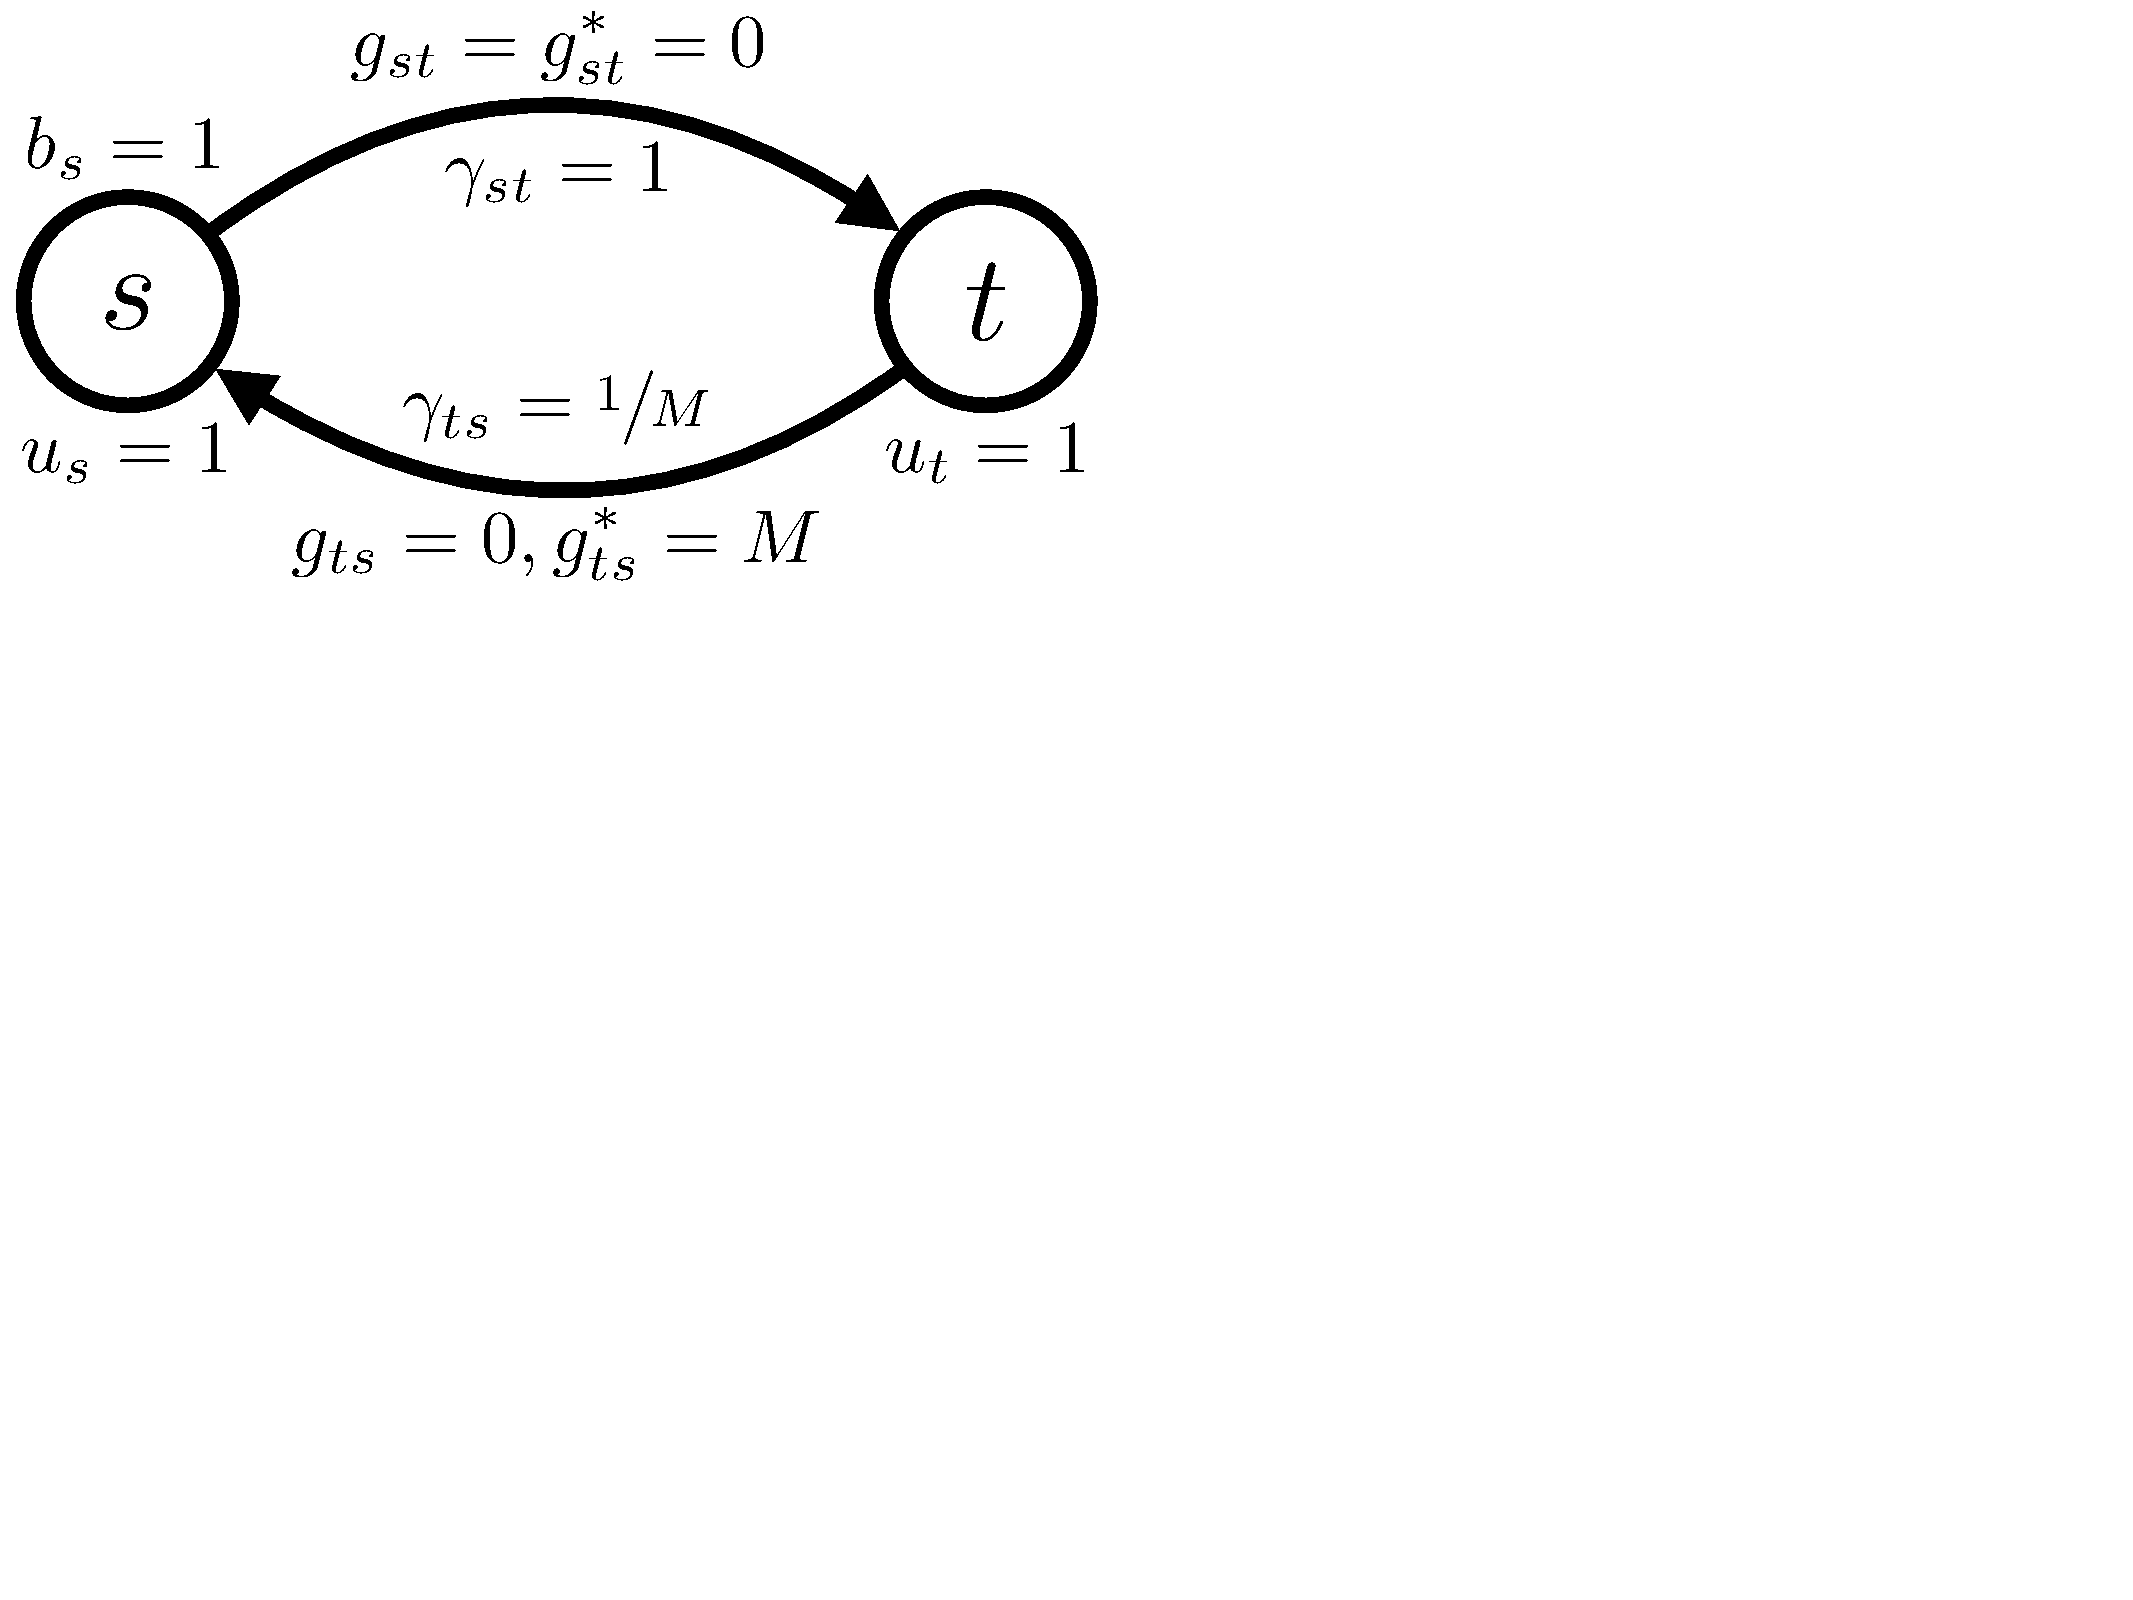
\includegraphics[width=0.45\textwidth]{figs/unsafe.pdf}
%    \caption{
%    \label{fig:unsafe}
%		If $\mu$ is not \textit{safe}, the distance between a $g$ fitting
%		$\mu$ and the optimal solution could be unbounded.
%    }
%    \end{figure}

%     Lemma \ref{lem.contractibility} shows that a fitting pair with a very
%     large flow value on one edge serves as a certificate that that edge is contractible.
%     To develop a strongly polynomial algorithm, it remains to show that we can compute
%     such a fitting pair.
    
    As outlined in Section \ref{sec:cert-contract}, the algorithm
    has a dual mandate---(i) bounding the relabeled excess and deficit and (ii)
    obtaining a large relabeled flow value on an edge. Both goals depend on the primal
    \emph{and} dual variables. As in Section \ref{sec:findcontr2013}, we can obtain
    a more useful contractibility certificate by disentangling the two. The following
    definition serves in place of abundant edge, and it only depends on the dual variables.
    \begin{definition}
    A node $i$ is \textbf{plentiful} with respect
    to the current primal-dual solution pair $(f,u)$ if its scaled absolute
    demand is large relative to the size of the graph: $|b_i^{\mu}| \ge 3n(d_i + 1)$.
    \end{definition}
	\begin{theorem} \label{thm:2017-contraction}
		Let $(f, \mu)$ be a fitting pair such that
		\begin{enumerate}[(i)]
			\item $\mu$ is safe.
			\item Excess is uniformly bounded: $\nabla f_i^\mu - \biu \leq 2$ everywhere.
			\item $i$ is a plentiful node.
		\end{enumerate}
		Then a contractible edge neighboring $i$ can be found in strongly polynomial time.
	\end{theorem}
	\begin{proof}
		First we compute a flow with bounded excess and deficit. Then we use it to obtain
		an abundant edge.
		
		Since $\mu$ is safe, there is some flow $f'$ satisfying $\biu \leq (f')_i^\mu$
		for all $i$ and $f'_e > 0$ only if $e$ is tight. Meanwhile, $\nfiu \leq \biu + 2$.
		By an ordinary maximum flow computation on the tight edges defined by $\mu$
		(\emph{cf.} \cite{Schrijver2002}, Corollary 11.2),
		it is possible to compute a flow $g$ which is not necessarily feasible but satisfies
		\[ \lfloor \biu \rfloor \leq \biu \leq \nabla (f')_i^\mu
		   \leq \nabla g_i^\mu \leq \nfiu \leq \max \{\nfiu, \lceil\biu\rceil\}. \]
		Clearly, $\Ex(g, \mu) \leq 2n$ and $\Def(g, \mu) \leq n - 1$. (Note that the
		sink $t$ is excluded from total excess and deficit.) Moreover, if $f$ is
		integral, then the outer bounds above are integral; so
		the computed flow $g$ will also be integral.
	
		Suppose that $i \in \vsrc$. (The other case is similar.) We have
		\[ \sum_{e \in \din(i)} g^\mu_e \geq
		\sum_{e \in \din(i)} g^\mu_e - \sum_{e \in \dout(i)} g^\mu_e
		= -\nabla g^\mu_i \geq -b_i^\mu - \Ex(g, \mu), \]
		where the last inequality is because $\nabla g_i^\mu - \biu$ appears
		as a term in $\Ex(g, \mu)$ if it is positive. Now
		\[ -b_i^\mu - \Ex(g, \mu) > 3n(d_i + 1) - 2n > 3nd_i > 3n|\dout(i)| \]
		So there is some edge $e \in \dout(i)$ with
		$g^\mu_e > 3n > \Ex(g, \mu) + \Def(g, \mu)$. This is an abundant and contractible
		edge.
	\end{proof}

	In practice, the algorithm maintains a fitting pair $(f, \mu)$ satisfying
	assumptions (i) and (ii) of Theorem \ref{thm:2017-contraction}. When it encounters
	a plentiful node $i$, it computes a new integral flow $g$ as described in the proof,
    uses it to identify
	an abundant edge neighboring $i$, and then contracts the edge.
	After contraction, $(g, \mu)$ is used to initialize the search for the next
	plentiful node.

%    It is important to notice that, just as with the definition of an abundant edge,
%    this definition depends only on the size of the graph, which is a key property
%    that will keep our algorithm strongly polynomial because we will be iteratively
%    re-scaling the node demands until one of them satisfies this property.
%
%    \begin{theorem} Assume $(f, \mu)$ is a fitting pair with $\mu$ safe.
%    Then the existence of a plentiful node $i$ ensures
%    that there exists a contractible edge $e$ incident to $i$.
%    \end{theorem}
%    \begin{proof} 
%    \todo{Prove theorem 3.1 more succinctly and clearly}.
%    \end{proof}

    \subsection{Producing a Plentiful Node}
    \label{sec:sub-ppn}
		%\frank{Replace any instances of "algorithm" in this section with "subroutine
		%to be clear}
		%\frank{When I used the term epoch here,
		%I was referring to the "subroutine" \textsc{Produce Plentiful Node} as an epoch,
		%as we don't give it a name anywhere else. The epochs are demarcated by contractions. Is
		%this incorrect? -- David}
		%The algorithm starts with a feasible fitting pair and consists of a sequence
    %of epochs, each dedicated to identifying a contractible edge via a plentiful node.
    %Each epoch alternates between the following augmentation and scaling
		%phases:\frank{we need to rewrite this. each epoch does not find a plentiful
		%node, there's only one produced at the end, we need to make this distinction
		%from the outer loop in the main algorithm where this is the case}
		In order to find a plentiful node for a fitting pair $(f,\mu)$, the algorithm uses a subroutine
		which alternates between the following augmentation and scaling phases until
		a node becomes plentiful:
    \begin{itemize}
    \item \textbf{Augmentation:} Reduce the total excess and deficit of the fitting flow $f$
    by augmenting as much flow as possible, one unit at a time, along tight paths from nodes with
		excess to nodes with deficit. We focus
		on tight paths because these are the highest-gain paths. Formally, let
    $D$ (``destinations'') be the union of the sink $t$ and all nodes with 
		deficit ($\nabla f_i^{\mu} < b_i^{\mu}$) and let $S$ (``sources'') be the
		set of all nodes $i$ for which $D$ is reachable from $i$ along a tight path
		in the residual graph. Continue augmenting along tight paths from $i$ to
		a node in $D$ as long as there is some $i \in S$ for which the following conditions hold:
		%Let $S$ (``sources'') be
    %the set of all nodes $i$ for which
    \begin{enumerate}[(i)]
    \item $i$ has at least one unit of excess ($\nabla f_i^{\mu} \ge b_i^{\mu} + 1$); and
    \item $b_i < 0$ (this condition is important in the potential analysis).
    \end{enumerate}
    %Augment until $S$ is empty.

    \item \textbf{Scaling:} Work toward producing a plentiful node by scaling the
    dual $\mu$ to increase $|b^\mu|$. Any excesses created during this
    phase must be cancelled by augmentation. In order to make this possible,
		only nodes in the set $S$ are scaled. 
    %the scaling only occurs in the set $S$ of reachable nodes.
    
    Notionally, a scaling factor $\alpha > 1$ is increased continuously, and
    $\mu_i \gets \mu_i / \alpha$ for $i \in S$.
    $\alpha$ increases until either there is a plentiful node in $S$ or some
    node in $S$ has an excess of at least $1$, triggering an augmentation phase.
    Flow on edges entirely within $S$ is also scaled by $f_e \gets f_e/\alpha$,
    so that $f_{ij}^\mu$ does not change when $i, j \in S$.
    
%    Once it is not possible to augment any more flow, the second step scales down
%    the labels and flow for all nodes and edges in $S$ by the same factor $\alpha$, 
%		\david{we do we only scale nodes in $S$? maybe have to be able to send
%		excess somewhere to be conservative and only scale things where you can
%		definitely send it }
%    which is chosen to be the smallest value that will allow us to make more
%		progress in the augmentation phase or produces a plentiful node. As we will
%		show below, this scaling strictly increases $|b_{i}^{\mu}|$ for $i \in S$
%		towards the definiton of a plentiful node.
    \end{itemize}
    
%    Although it is not necessary in practice, for clarity of explanation, one
%		can think of choosing the scaling factor $\alpha$ as solving the following LP:
%    \lpeq{\lpthree{max}
%    {\alpha}
%    {\gamma_{ij}^{\mu} \le 1\ \forall\ i,j \in \din(S)}
%    {\nfiu - \biu \le 1}
%    {\nexists\ \text{plentiful}\ i \in \vsink}
%    }\frank{Change this to be actual condition of plentiful node that way it can
%	become tight and add some insight in the text about this.}
%
%
%
%    \begin{figure}[b!]
%    \centering
%    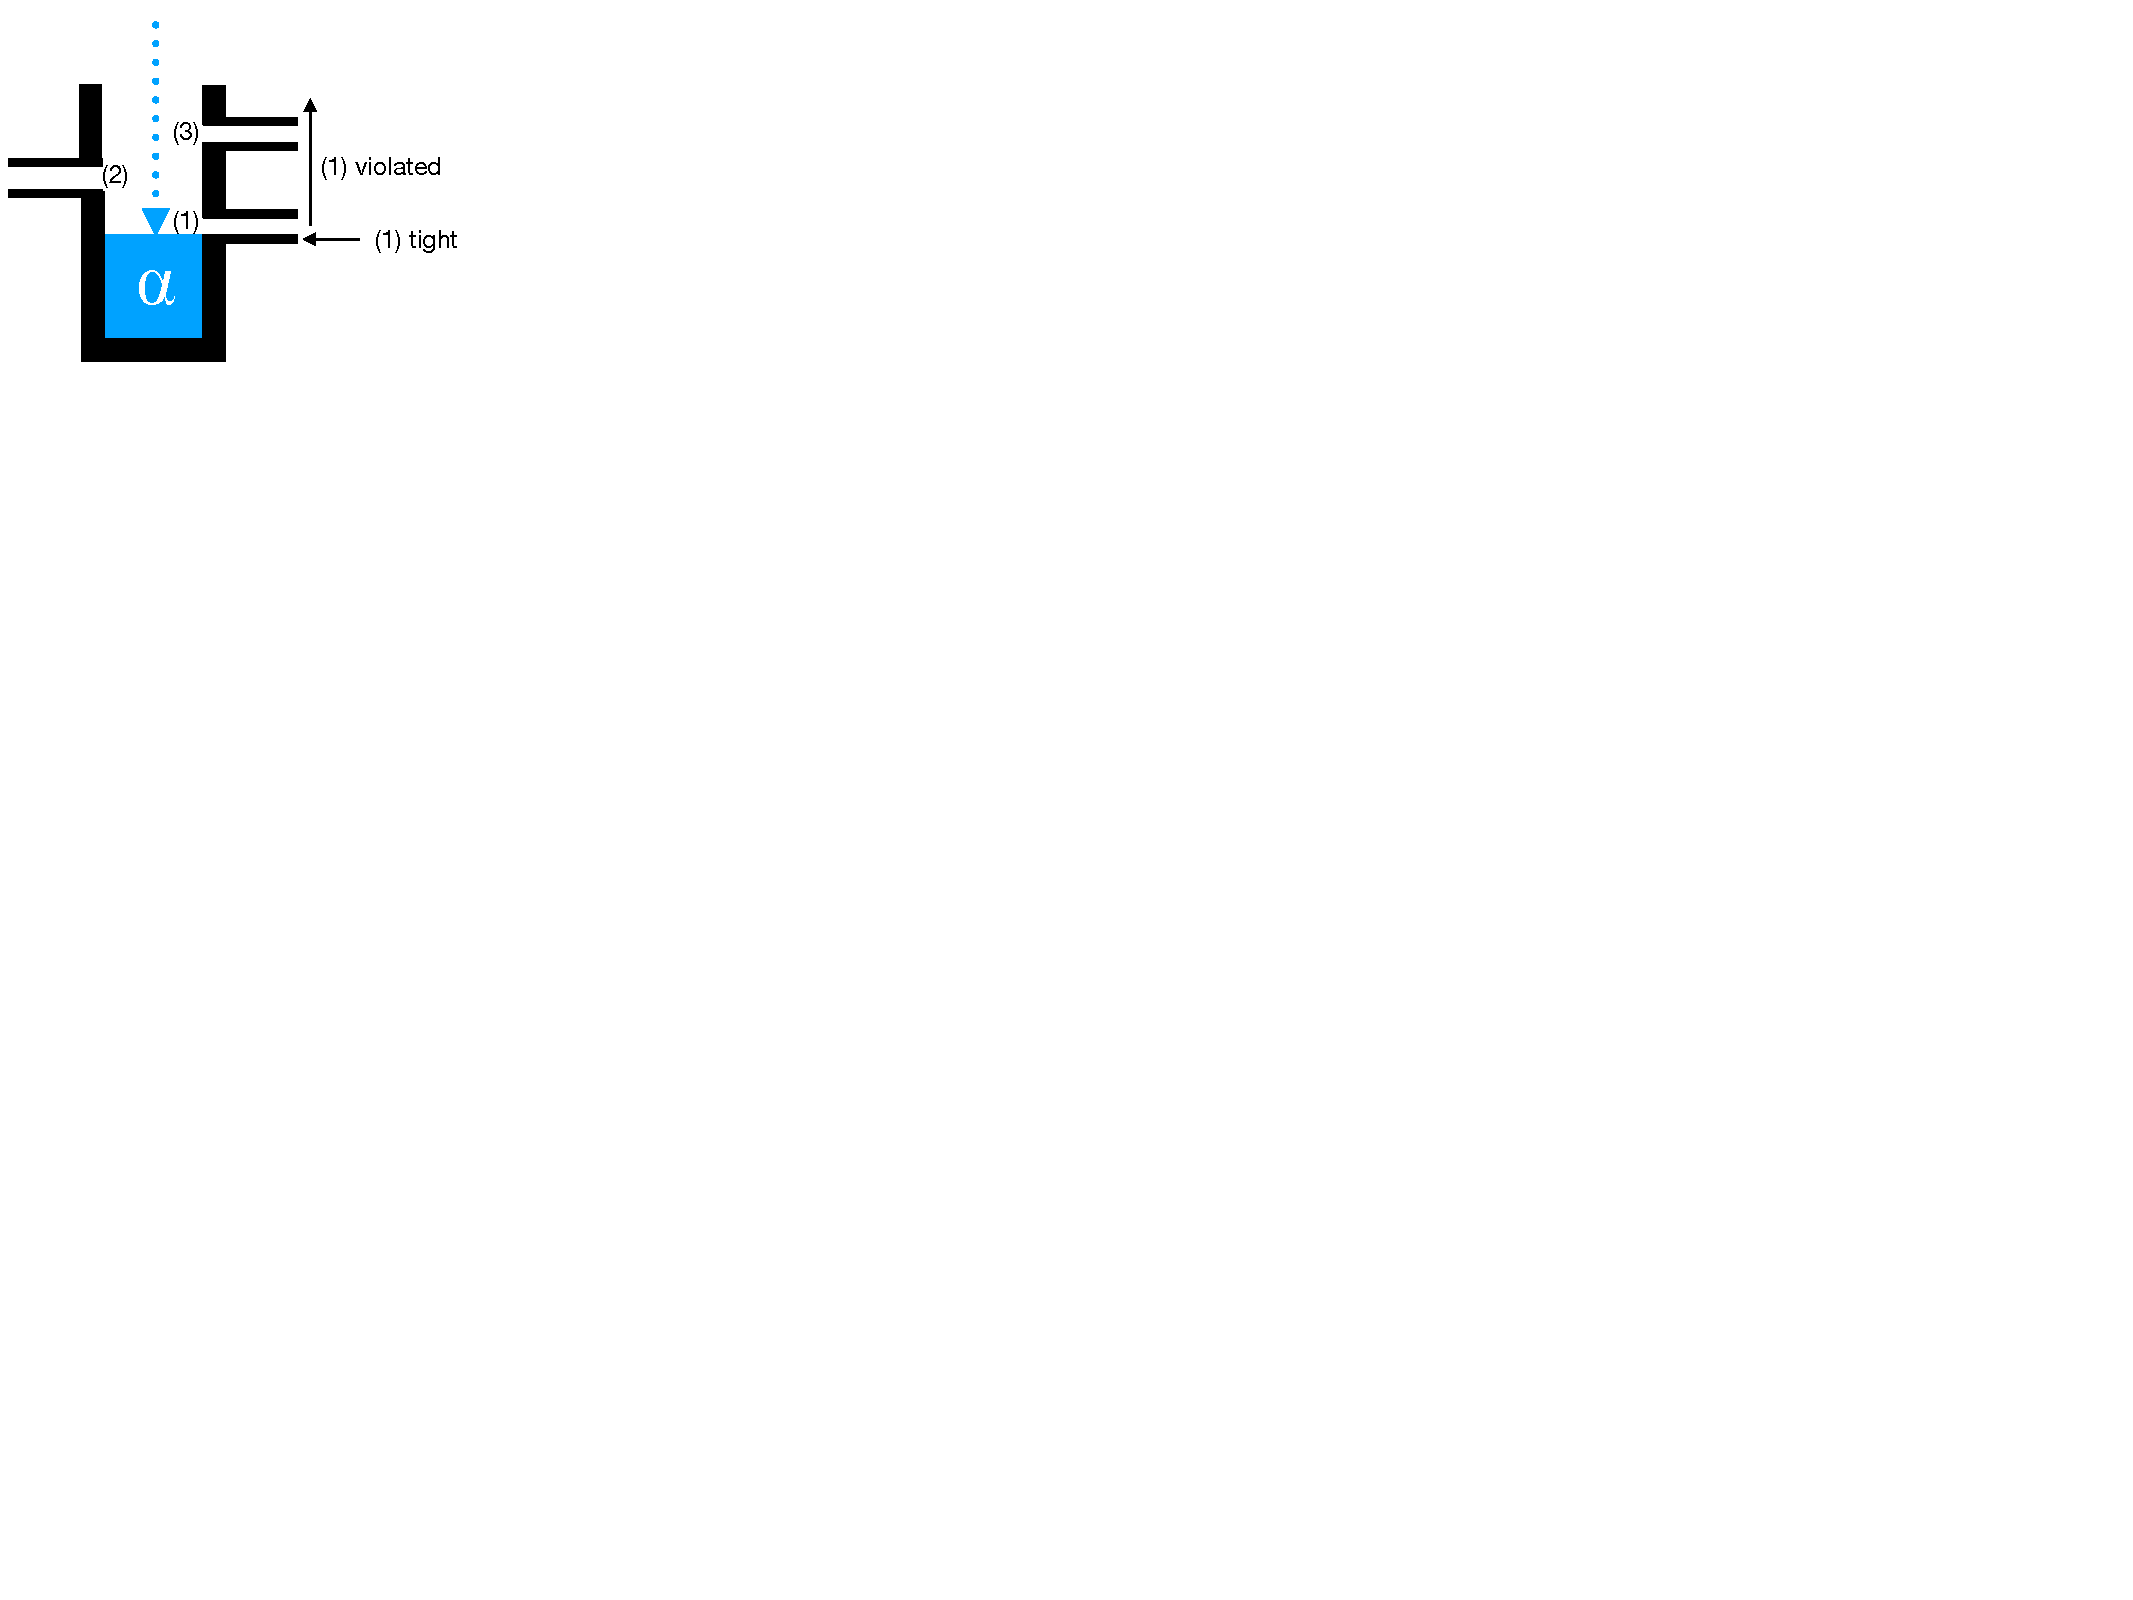
\includegraphics[width=0.35\textwidth]{figs/water.pdf}
%    \caption{
%    \label{fig:alpha}
%    Informal analogy for the maximization of scaling parameter $\alpha$.
%    Each pipe represents a constraint. $\alpha$ can only be increased until
%    one of them becomes tight as increasing it further would leak into
%    the lowest pipe and violate that constraint.
%    At each step, the order of which constraint becomes tight first may be different.
%    }
%    \end{figure}
%    Intuitively, as illustrated in Figure~\ref{fig:alpha}, this is akin to filling
%    a basin with water as much as possible without any of the water leaking into one
%    of three pipes, where each pipe represents a constraint and its height in the basin
%    represents the value of $\alpha$ at which point it becomes tight.
%
%    Thus, $\alpha$ is chosen such that one of the following constraints becomes
%    tight, or, in other words, one of the following becomes true corresponding to
%    each constraint, respectively:
%    \begin{enumerate}[(1),itemsep=-1mm]
%        \item An edge entering $S$ becomes tight, and thus a new node is added to $S$
%        \item A node in $S$ has excess $>1$, which allows us to augment flow from it
%        \item A node becomes plentiful
%    \end{enumerate}
%
%    If (3) is true, we're done. If (1) or (2) are true, it ensures that we will now
%    be able to make progress in the next iteration of the first step. Below, we show
%    in Lemma~\ref{lem:scaling} that the augmentations in the first step similarly ensure
%    that the algorithm can make progress in the second step.

	Intuitively, scaling is
	akin to filling a basin with water. As illustrated in
	Figure~\ref{fig:alpha},	imagine a basin with various levels,
	where the height of the water represents $\alpha$ and each
	level corresponds to a vertex on the boundary of $S$. The area under water
	represents $S$.
	As $\alpha$ rises, an incoming edge $(i, j)$ becomes tight. This in turn
	causes $i$ to be added to $S$, as $S$ is now reachable along a tight
	path from $i$. Updating $S$ during scaling maintains the invariant that
	$S$ is inward-loose.
    \begin{figure}[b!]
    \centering
    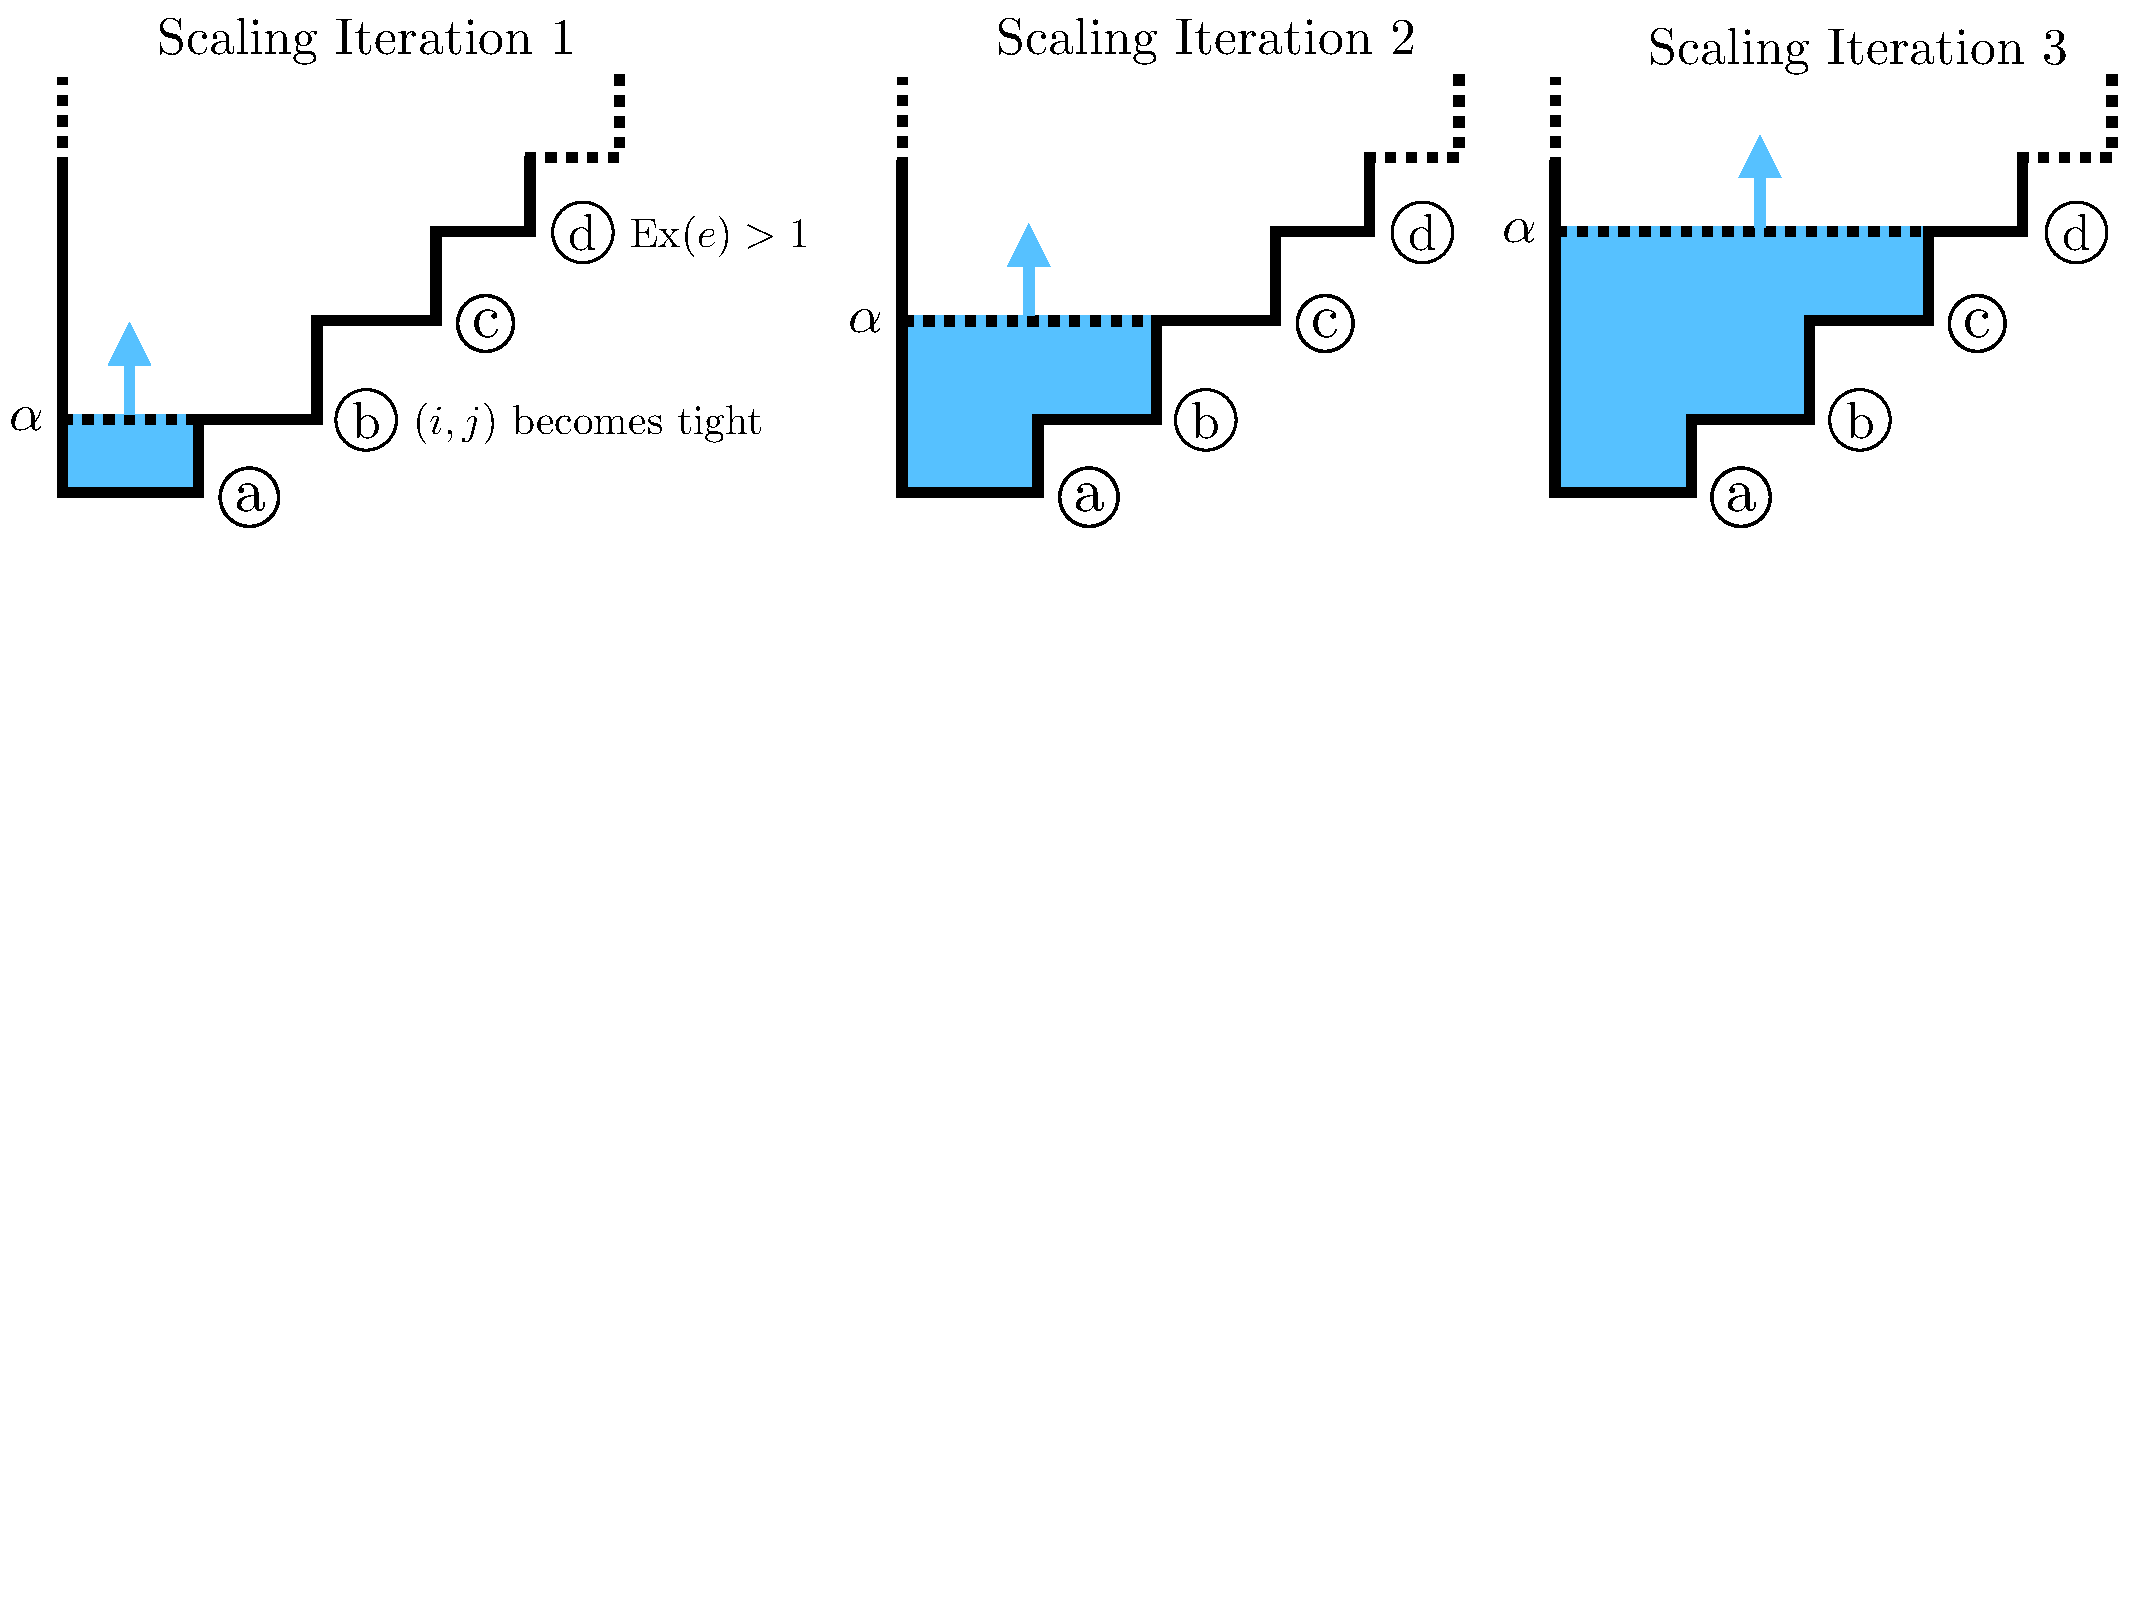
\includegraphics[width=\textwidth]{figs/alpha.pdf}
    \caption{
    \label{fig:alpha}
		Informal analogy showing how the dual is scaled at each iteration just
		enough to keep the dual feasible and the primal bounded.
    }
    \end{figure}
		
%	Scaling $\alpha$ past one of these points in a single iteration would break the constraint.
%	Thus, at each scaling step, we can only increase $\alpha$ by at most one
%	level in the basin.
%	For example, consider point (b) where the incoming edge $(i,j) \in \din(S)$ becomes tight.
%	Increasing $\alpha$ past this point would cause $\gamma_{ij}^{\mu}$ to be
%	greater than 1, breaking the the feasibility of the dual. Setting $\alpha$
%	to exactly this value will make the edge tight, meaning we can add $i$ to our
%	list of potential augmentation sources $S$. Expanding $S$ helps, but we
%	cannot actually augment until a node in $S$ has excess at least 1. However,
%	we do not want to scale $\alpha$ past this point because, as described in
%	Section~\ref{sec:contract-cert},
%	\david{Perhaps bring this point out more in 5.2 if necessary}
%	we need to keep the primal bounded. Thus, we
%	continue filling the basin one step at a time until we reach this condition
%	(e.g. at point (d)), or the stopping condition where the plentiful node
%	constraint becomes tight.

    In practice, $\alpha$ and $S$ can be updated via a modified Dijkstra's algorithm.
    Let $c_{ij} = - \log \gij$ be the ``cost'' of edge $(i, j)$.
    Then $(i, j)$ is tight exactly when
    \[ c_{ij} = \log \mu_i - \log \mu_j. \]
    In other words, tight paths are shortest paths, $\log \mu$ is a distance function,
    and $S$ is a ``frontier.'' Scaling $\mu$ by $\alpha^{-1}$ in $S$ amounts to adding
    $\log \alpha$ to the distance of every node in $S$. Each new node added to $S$
    is the closest node under the costs $c_{ij}$, and it is encountered when $\log \alpha$
    reaches its distance.
    Dijkstra's algorithm with costs $c_{ij}$ will compute the maximum distance $\log \alpha$,
    and it can be terminated when either a plentiful node or an excess greater than
    one is encountered.

	\subsection{Analysis}
	We now demonstrate some invariants preserved by the algorithm. In particular,
	we show that the algorithm maintains assumptions (i) and (ii) of
	Theorem \ref{thm:2017-contraction}, so that a plentiful node guarantees the
	existence of a contractible edge.
    \begin{lemma}
    Relabeled flow $f^{\mu}$ remains unchanged during each epoch.
    \label{lem:fsame}
    \end{lemma} 
    \begin{proof}
			As seen above, the scaling is designed so that $f_{ij}^\mu = f_{ij}/\mu_i$
			stays constant when both $i$ and $j$ are in $S$. Moreover, it maintains the
    	invariant that there is no flow across the cut $S$---so flow across $S$ is vacuously
    	preserved under scaling. Finally, scaling does not affect edges entirely
    	outside $S$.
    \end{proof}
    \begin{corollary}
    $f^{\mu}$ is always integral.
    \end{corollary}
    \begin{proof}
    The flow is initially rounded to be integral (Section \ref{sec:2017-rounding} below). 
    The augmentation step clearly maintains integrality of $f^{\mu}$ because we
    always augment by 1 unit at a time. By
    Lemma~\ref{lem:fsame}, scaling never changes the value of $f^{\mu}$ at all.
    Finally, at a contraction, a new integral flow is computed.
    \end{proof}
%    \begin{lemma}
%        \label{lem:scaling}
%        For all nodes with non-zero demand in $S$, scaling $\mu$ in the second step
%        strictly increases $|\biu|$. For all other nodes, $|\biu|$ remains unchanged.
%        \todo{Show S cannot be empty?}
%    \end{lemma}
%    \begin{proof}
%        First, trivially, scaling a node with zero demand cannot change its value
%        ($0\cdot\mu=0$), and the algorithm only updates $\mu_i$ for $i \in S$. Recall
%        that $\biu$ is defined as $b_i / \mu_i$, and thus, if $\mu_i\leftarrow \mu_i / \alpha$,
%        then
%        \[ \biu \leftarrow \frac{b_i}{\mu_i / \alpha} = \alpha\frac{b_i}{\mu_i} = \alpha \biu. \] 
%        Now it suffices to prove that $\alpha > 1$ always holds when any of the three
%        constraints become tight.
%
%        By construction, before rescaling, $S$ has no tight
%        incoming edges. Recall $\giij = \gamma_i\frac{u_i}{u_j}$. In order for an
%        incoming edge $i \notin S, j\in S$ to become tight (1), we must have $\giij=1$:
%        since we only scale values in $S$, $\alpha$ must be ${1}/{\giij}$, which is
%        always greater than $1$ because $\giij < 1$ (by the feasibility of the dual).
%
%        From the terminating condition of the augmentation step (the lack of any nodes
%        in $S$ having excess), we know $\Ex(f) = \nfiu - \biu < 1$. Since, by
%        Lemma~\ref{lem:fsame}, $\nfiu$ is unchanged and only nodes in $\vsrc$ (i.e. $b_i<0$)
%        can have excess, the only way for to make $\Ex(f) \ge 1$ is if $\biu$ becomes
%        more negative, which only happens if $\alpha > 1$. 
%
%        Finally, we start out with the assumption that there are no plentiful nodes.
%        In order for a node to become plentiful (3), its demand $\biu$ must increase,
%        which is only possible if $\alpha > 1$.
%    \end{proof}
    \begin{lemma}
        \label{lem:still-fit}
        $\fp$ remains a fitting pair throughout each epoch.
    \end{lemma}
    \begin{proof}
    Suppose that, at the beginning of the epoch, $f$ fits $\mu$. That is, $\mu$
    is dual-feasible, and whenever
    $f_{ij} > 0$, $\giij = 1$. Augmentation only occurs along tight edges, thus
    maintaining the fitting property. Scaling only changes $\giij = \gij \mu_i / \mu_j$
    when $(i, j)$ crosses between $S$ and $V \setminus S$. But there is no flow crossing
    this cut, so scaling never violates the fitting property. Moreover, as soon as an edge
    crossing the cut becomes tight, $S$ is expanded. Thus, the constraint
    $\giij \leq 1$ is never violated during scaling, i.e., $\mu$ remains feasible.
    \end{proof}

    \begin{lemma}
        $\mu$ remains safe throughout each epoch, i.e. there is a corresponding feasible primal
        solution even though we haven't kept track of it.
    \end{lemma}
    \begin{proof}[Proof Sketch]
	Only the scaling steps modify $\mu$, so it suffices to show that one scaling step,
	during which at most one node is added to $S$,
	preserves safety. Assume that $\mu$ is initially safe, and
	assume by way of contradiction that the updated labeling $\mu'$ is no longer safe.
    That is, there exists some inward-loose cut $X \subseteq \vnott$
    with net positive demand $b^{\mu'}(X) > 0$.

    Divide $X$ into $X \cap S$ and $X \setminus S$, where $S$ is defined by the original
    $\mu$.
    Recall that scaling only affects $X \cap S$, so we can write the net demand under $\mu'$
    in terms of the demands under $\mu$ as follows:
    \[ b^{\mu'}(X) = \frac{1}{\alpha}b^{\mu}(X \cap S) + b^{\mu}(X \setminus S) \]
    Either $b^{\mu}(X \cap S)$ or $b^{\mu}(X \setminus S)$ must be positive.
    
    Suppose $b^\mu(X \cap S) > 0$.
    Observe that $\din(X \cap S) \subseteq (\din(X) \cap E[S]) \cup \din(S)$, where $E[S]$
    denotes the edges entirely inside $S$.
    By definition of $S$, $\din(S) \cap \tau(\mu) = \varnothing$. Moreover,
    $E[S] \cap \tau(\mu) \subseteq E[S] \cap \tau(\mu')$. So
    \[ \din(X) \cap E[S] \cap \tau(\mu) \subseteq \din(X) \cap \tau(\mu) = \varnothing. \]
    So $X \cap S$ is an inward-loose cut with positive net demand under $\mu$, contradicting
    the safety of $\mu$.
    
    The case where $b^\mu(X \setminus S) > 0$ is similar, though slightly more complicated.
    \end{proof}

    In summary, we have shown that the primal and dual steps always allow room for the other to make progress, and collectively each iteration of the two steps strictly increases $|\biu|$ towards
    the definition of a plentiful node. Thus, the subroutine will eventually produce one. We have also shown that the updates it makes to $f$ and $\mu$ do not violate any of the previous conditions stated for being able to ultimately derive a primal optimal solution once our fitting pair finds the dual optimal. 

\iffalse
	 \subsection{Finding a feasible flow}
	\todo{Don't they just run the whole algorithm on a modified graph to initialize?}
	Drawing inspiration from the Simplex algorithm, the first step in this algorithm is finding a trivial feasible solution $(\bar{f}, \bar{\mu})$, which clearly also satisfies the definition of a fitting pair necessary for the algorithm. In order to find this initial solution, rather than using Radzik's cycle-cancelling subroutine as in prior work, the authors develop a new method based on negative cycle detection, which can be run in $O(nm)$ time. \todo{references} 
    \fi
    
    \subsection{Initialization} \label{sec:2017-rounding}
	The algorithm needs to start with a fitting pair $(f, \mu)$ where $\mu$ is safe,
	$f$ is integral, and $f$ has bounded excess,
	as required in Theorem \ref{thm:2017-contraction}.
	
	To do this, the algorithm starts by computing a conservative pair $(\bar{f}, \mu)$,
	thus ensuring
	that $\mu$ is safe. This feasibility problem can be solved by running the same
	generalized flow algorithm on a carefully constructed graph whose optimum is a feasible
	solution to the original problem. This is akin to the way the
	simplex algorithm is initialized.
	
	Next, $\mu$ is scaled so that the relabeled excess is uniformly bounded.
	Then, the flow
	is ``rounded'' to be integral by computing an ordinary flow $f^\mu$ on the tight edges
	defined by $\mu$ under the constraints
	\[ \lfloor \nabla \bar{f}^\mu_i \rfloor \leq \nfiu
	 \leq \lceil \nabla \bar{f}^\mu_i \rceil. \]
	The result is a fitting pair such that $f^\mu$ is integral and satisfies
	\[ \biu - 1 \leq \nfiu \leq \biu - 2. \]
	The first epoch begins with this fitting pair.

    \subsection{Running Time Analysis}
    The algorithm consists of three basic types of operations: scaling, augmentation, and contraction.
    The number of contractions is bounded by $n$. Contraction itself
    requires computing a regular flow and performing a bounded number of graph operations, but
    strongly polynomial algorithms already exist for these. So the goal is to bound the running time
    (number of arithmetic operations) between any two contractions.

    Augmentation itself consists of a graph search on the tight subgraph, an $O(m)$ operation.
    Between rounds of augmentation, there is a scaling round. Each scaling phase stops
    when either (i) a node has become plentiful, leading to a contraction, or (ii) a node has an
    excess greater than $1$, leading to a new augmentation round.
    If the scaling is done by Dijkstra's algorithm as
    described in Section \label{sec:sub-ppn},
    the cost of each scaling phase (and thus the overall cost per augmentation) is
    $O(m + n \log n)$.

    It remains to bound the total number of augmentations the algorithm may perform. We'd
    like to show that after a strongly polynomial number of augmentations, the algorithm
    is guaranteed to find a plentiful node.

    \begin{lemma} \label{lem.num-aug}
        After $O(mn)$ augmentations, the algorithm is guaranteed to find a plentiful node.
    \end{lemma}
    First, a preliminary lemma. We denote the period between successive contraction
    steps as an epoch.
    \begin{lemma} \label{lem:deficit-bound}
    At any node $i \in \vsrc$, the deficit is at most one. Moreover, at most one augmentation
    ends at such a node during any epoch.
    \end{lemma}
    \begin{proof}
        At the beginning of the algorithm, the flow is feasible, so $\nfiu - \biu \geq 0$.
        Rounding decreases $\nfiu$ by less than one. Similarly, during each contraction,
        the adjusted flow is computed with $\nabla g_i^\mu \geq \lfloor \biu \rfloor$ everywhere.

        Between contractions, the deficit can be modified by scaling and augmentation steps.
        Since $i \in \vsrc$, $\biu < 0$, and so $\biu$ can only decrease during scaling.
        Meanwhile, augmentations only decrease deficits.
        Once $\nfiu \geq \biu$, no augmentation ending at $i$ will be contemplated unless $i$
        experiences a deficit again. The only way for this to happen would be for
        augmentations beginning at $i$ to reduce $\nfiu$ below $\biu$. However,
        an augmentation will only begin at $i$ if
        $\nfiu - \biu \geq 1$, and will reduce $\nfiu$ by exactly one. Hence, $i$ will
        never again experience a deficit during the epoch, and so there will be no further
        augmentations ending at $i$.
    \end{proof}

    \begin{proof}[Proof of Lemma \ref{lem.num-aug}]
    Define two potential functions
    \begin{align*}
    \Psi(\mu) &= - \sum_{i \in \vsrc} \biu \\
    \Phi(f, \mu) &= \sum_{i \in \vsrc} \nfiu + \Psi(\mu) = \sum_{i \in \vsrc} \nfiu - \biu
                 \leq \Ex(\mu)
    \end{align*}
    By Lemma \ref{lem:deficit-bound}, $\Phi(f, \mu) \geq -\Def(f, \mu) \geq -n$
    throughout the algorithm. Similarly, $\Phi(f, \mu) \leq \Ex(f, \mu) \leq 2n$.
    Finally, it follows from Lemma \ref{lem:deficit-bound} that at most $n$ augmentations
    may end in $\vsrc$, thus not decreasing $\Phi$. So after $r$ augmentations,
    $\Phi$ has decreased by at least $r - n$. Its total decrease is bounded by $2n - -n = 3n$,
    so there must be a corresponding increase of at least $r - 4n$ during scaling. So
    $\Psi$ also increases by at least $r - 4n$, as $f^\mu$ is constant under scaling.
    
    Therefore, after $O(mn)$ augmentations, $\Psi$ is sufficiently large so as to guarantee
    the existence of a plentiful node in $V^s$.
    \end{proof}
    We have shown that there are at most $n$ epochs of $O(mn)$ augmentations each, with
    each augmentation costing $O(m + n\log n)$. This implies an $O(mn^2(m + n\log n))$
    time bound overall. With a more careful potential analysis, the bound can be improved
    to $O(mn\log(n^2/m)(m + n \log n))$.


\section{Conclusion}\label{sec:discussion} 

We presented and compared two strongly polynomial algorithms for the maximum generalized flow problem.
Both algorithms take a combinatorial solution by computing a set of tight edges consistent
with an optimal dual solution. In both cases, this set is built up inductively by
contracting edges. Finally, in both cases, a pair of primal and dual solutions is used to
construct certificates of contractibility.
Olver and Végh \cite{Olver2017} achieve an improvement of almost $O(n^2)$ by relaxing the
feasibility of the primal flow component of the pair. This allows excess to be cancelled with deficit,
making it much easier to keep both bounded and thus reducing the time required to find each
contractible edge.

%	\subsection{Non-triviality of a strongly polynomial algorithm}

%	\todo{Explain} why applying ideas from strongly polynomial algorithms for
%	min-cost flow was not straightforward. 

%	We know that the feasibility problems are the same for min-cost and
	%generalized max-flow. Min-cost objective is additive: when you change the
	%value of the flow on one edge, that doesn't affect the objective piece for any
	%other edge, whereas in the
    

\setlength{\bibitemsep}{0pt}
\nocite{*}
\printbibliography
\end{document}
 
